\chapter{基于触发器的计算模型}
\label{chapter:domino}

\section{引言}

大数据时代的到来,人们每天搜集和存储的数据越来越多。这些数据中包含了各种有用的信息。比如电子商务网站会记录用户浏览历史,甚至浏览时鼠标停留的位置和时间。对每一个用户来说,这些记录的数据量并不大,但是对于通常拥有上亿用户的电子商务网站来说,记录这些数据就需要足够的资金来建立海量存储系统。企业愿意付出巨大成本来记录这些信息,是因为这些数据确实能为公司带来利润。利用这些数据对用户行为进行分析,能够非常准确的识别出每一个用户的特征、喜好、需求,并且针对性的给予商品推荐,从而提高推荐到购买的转化率。当然,除了存储处理这些本身就在赛博空间(Cyber Space)产生的数据之外,越来越多物理世界的数据也开始被数字化、收集并且加以利用,比如实时交通路况数据,街景信息,停车位信息,甚至是热门饭店的排位信息。在这些数据被存储之后,更重要的就是如何处理以利用他们。

大量像Amazon EC2或者Windows Azure等IaaS基础设施服务的出现使得按需获取大规模计算资源成为可能,这也使得利用这些海量的数据成为可能。然而,正如过去几十年计算机的发展所揭示的那样,设计和实现不同种类的可扩放的应用程序依旧非常困难,特别是对于需要大规模计算的领域专家而言,他们除了需要考虑应用本身的分布式实现之外,还需要考虑竞争条件、死锁、分布式状态管理、同步等非常复杂的技术问题。为了把应用开发人员和这些繁琐复杂的分布式问题分隔开来,大量的分布式计算模型开始出现。我们认为一个分布式的计算模型包括编程模型、运行时系统支持、容错恢复、任务调度、多用户管理等几个部分。

在现有云计算平台的多种计算模型的基础上,本章将介绍一种基于触发器的新型云计算平台中的计算模型——Domino。该计算模型包括了编程模型、运行时支持、以及容错恢复等部件,并且通过与现有的云计算存储系统整合,为开发人员提供了一个简单、直观、高效的大规模应用开发的计算模型。Domino通过整合HBase存储系统来为应用开发人员提供了完整的存储和处理基础设施以便用户更加容易的编写那些包含了大规模的迭代和递增处理的应用程序。

我们基于Domino模型实现了一系列示例应用,如PageRank、一些比较典型的机器学习和数据挖掘算法($K$-means, 协同过滤)、分布式的爬虫等。通过这些应用的编写和性能对比试验,我们认为Domino在递增计算场景下具备了比现有的云计算模型更为简单有效的处理能力。相比较传统的MapReduce以及其扩展模型,具有了更高的计算效率和简洁的编程抽象,更重要的是,Domino还为我们的大规模分布式应用程序提供了实时的容错恢复能力,这一点是现有的模型很难做到的。

本章将首先介绍现有的编程模型以及问题,详细的介绍基于触发器的编程模型。\ref{section:intro}节,我们将综合一个分布式爬虫的例子来介绍什么叫做\textit{基于触发器的}编程模型以及为什么使用触发器模型来进行编程;在\ref{section:sync}节,我们将着重介绍Domino中的同步模型;\ref{section:design}节具体的介绍Domino的实际设计与实现的细节;\ref{section:apps}节结合几个典型的应用介绍如何在Domino中实现不同种类的应用;最后在\ref{section:exp}节通过一系列的性能对比来验证Domino本身的性能以及其上运行的应用程序的性能。

\section{相关工作介绍}

\subsection{MapReduce模型及其问题}

MapReduce自从2006年由Google提出,之后由Apache基金会以Hadoop项目开源实现,当前已经成为云计算平台中的标准配置。作为一个批处理的计算模型,MapReduce非常适合于进行日志分析、离线推荐算法。然而MapReduce依旧存在很多问题:
\begin{enumerate}
\item 不能很好的支持小的任务或者交互式任务。来自Google的统计数据,一个MapReduce任务平均需要8分钟的时间来执行,而一个PageRank算法重新运行一轮甚至需要几天的时间。这导致现有的MapReduce十分不适合以下几种任务:实时搜索、在线推荐或者广告系统。可惜的是这些应用恰好是互联网收入的主要来源。再比如,在线推荐系统中,我们需要根据当前用户点击和浏览数据来计算新的推荐数据,这应该在几秒内实现。很明显的,现有的MapReduce是不符合的。

\item 不适合迭代式的数据处理。许多数据分析技术都需要交互式计算,包括新型的PageRank算法,HITS(Hypertext-Induced Topic Search),递归关系查询,神经网络分析,社交网络分析等。这些技术都有一个共同的特点:数据都是被迭代处理,直到计算收敛或者到达停止条件。MapReduce不能很好的支持这种迭代式的数据分析程序,开发人员只能通过编写驱动程序来手动的启动和管理多轮MapReduce工作。而这种开发方式显然不是一个好方法,1),每一轮迭代中,数据必须不断的重新载入,重新处理,这将极大的浪费I/O,网络带宽和CPU资源;2),停止条件或者收敛判断往往还需要一个额外的MapReduce来进行判断,这将引入非常大的延迟。

\item	MapReduce不适合进行数据源不断增加的分析任务。许多数据分析技术都需要对数据集进行递增计算,比如实时搜索引擎使用PageRank算法来对所有抓取到的页面排序,当爬虫爬取到部分新增网页,如果对所有页面一起运行完整的PageRank算法则极大的浪费了计算资源。可惜的是,这正是当前的实际情况。

\item 使用MapReduce的编程框架,应用程序不能在线访问计算的任何中间状态,只能通过将不同的数据流进行聚合来模拟传统的共享内存结构。

\end{enumerate}

为了解决这些问题,人们提出了许多改进和设计,我们将首先介绍其中的典型代表,并最终介绍基于触发器的计算模型。

\subsection{迭代处理模型}

HaLoop\cite{bu2010haloop}是一个基于Hadoop MapReduce模型针对迭代任务的改进版本。HaLoop不仅仅通过扩展MapReduce模型使其支持迭代应用,并且提出了迭代感知的调度器以及引入了迭代任务之间的缓存,极大的提高了迭代应用的执行效率。

\begin{figure}[h!]
\centering
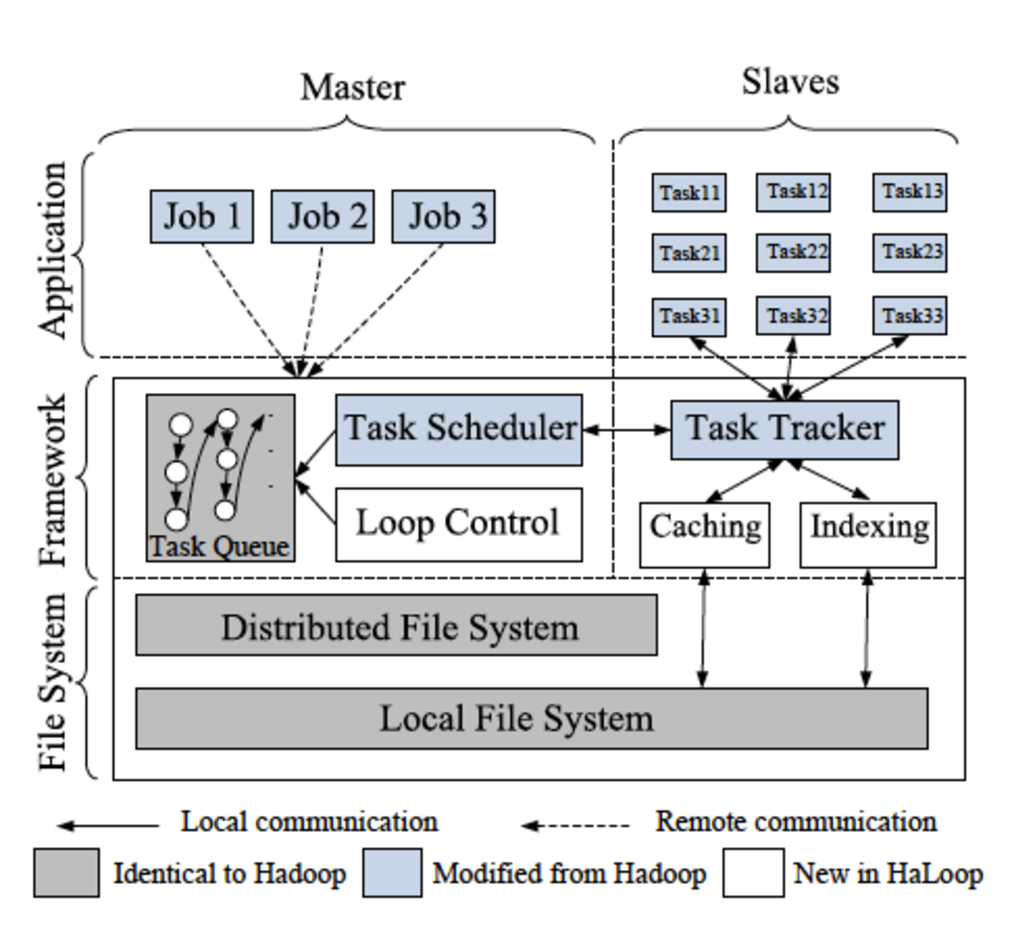
\includegraphics[width=4in]{../figures/haloop.pdf}
\caption{HaLoop架构图}
\label{fig:haloop}
\end{figure}

图\ref{fig:haloop}展示了HaLoop的整体架构。与Hadoop架构非常类似,HaLoop集群中包括了一个主节点和若干个从属节点。客户端向主节点提交任务,对每一个提交的任务,主节点会建立并且调度一系列子任务并发的在从属节点上执行。与Hadoop架构不同主要体现在,HaLoop的主节点包含了一个循环控制模块(Loop Control),能够不断的自动启动用户写入在循环体内的map-reduce任务直到用户指定的循环条件不再满足自动停止;其次,Haloop使用了新的任务调度器,该调度器能够感知到迭代计算的任务,并且通过将数据优先调度到数据所在的节点来提高数据的局部性。最后,HaLoop能够主动的在从属节点中缓存迭代过程中产生的不变量,同时也会缓存reduce的输出以加速下一个迭代的执行速率。

Haloop支持的迭代程序可以用下面的公式来描述:
\begin{equation}
R_{i+1}=R_0 \cup (R_i \bowtie L)
\end{equation}
其中$R_0$代表初始的结果,L代表计算过程中的不变量。

在HaLoop中编写程序时候,程序员应当指定循环体、循环终止条件以及循环不变量。为了帮助编程人员实现终止条件,Haloop提供了一些函数:\textit{SetFixedPointThreashold, ResultDistance, SetMaxNumOfIterations...}来提高编程效率。


Twister\cite{ekanayake2010twister}是另外一个支持迭代计算的MapReduce模型扩展。不同于Haloop,它使用了一种基于\textit{publish/subscribe}的消息传递的架构来进行数据传输和通讯以支持那些\textit{长时间运行}的mapreduce任务。

\begin{figure}[h!]
\centering
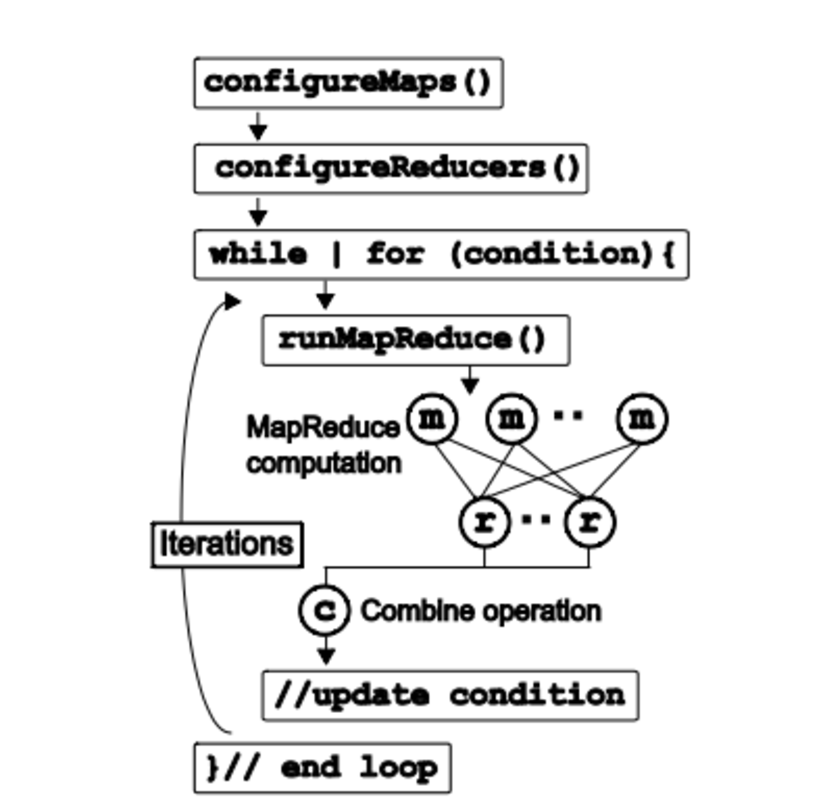
\includegraphics[width=3in]{../figures/twister.pdf}
\caption{Twister下迭代MapReduce编程模型示意图}
\label{fig:twister}
\end{figure}

图\ref{fig:twister}描述了Twister的扩展计算模型。Twister为MapReduce任务引入了配置阶段,在这个阶段里用户可以加载任何的静态数据以供后面的map和reduce阶段使用。那些长时间运行的mapreduce会将这些静态数据加载入内存以供迭代中不断使用。

图\ref{fig:twisterarch}进一步描述了Twister运行时的具体架构,其主要包括三个组件:1)客户端驱动程序,驱动了整个迭代程序的执行;2)所有的worker节点上运行的Twister守护进程;3)Broker网络节点。所有的worker节点启动后Twister守护进程会向Broker网络发起连接请求来接受命令和数据,该守护进程负责管理分配给自己的map和reduce任务,通知节点状态,并且最终需要对控制命令给予合适的响应。客户端驱动程序为用户提供了编程API并且将用户提交的API调用转变为控制命令和输入数据通过Broker网络发送给worker节点。

\begin{figure}[]
\centering
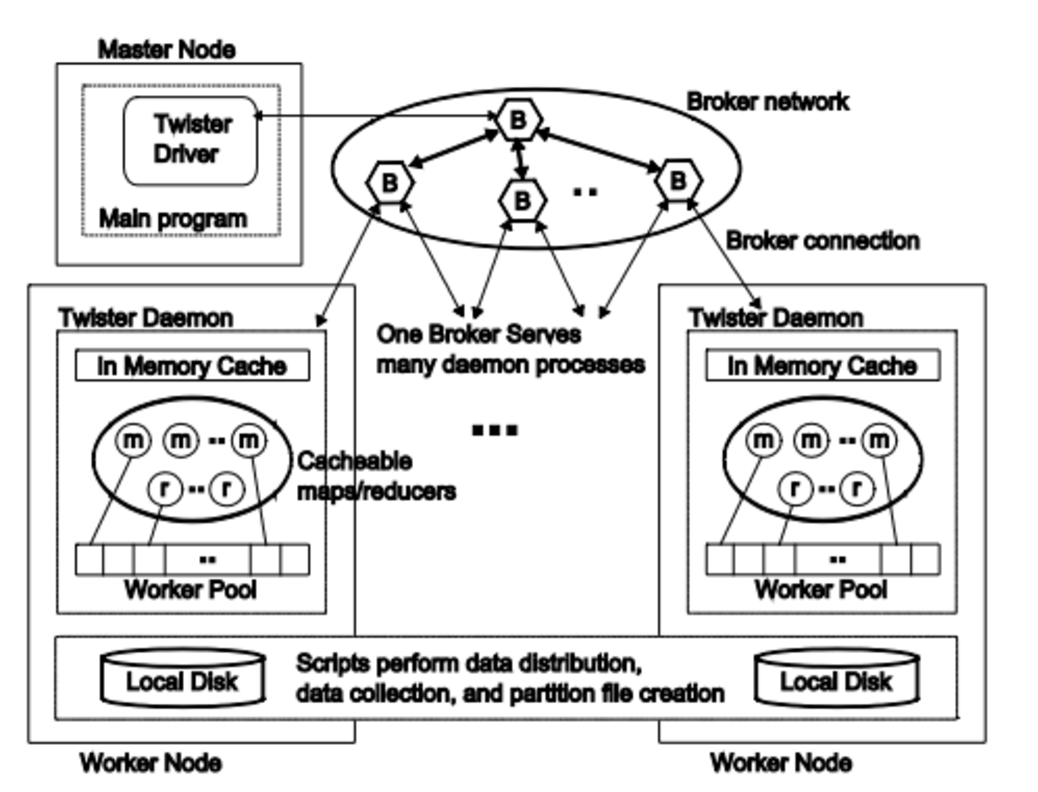
\includegraphics[width=4in]{../figures/twisterarch.pdf}
\caption{Twister系统的总体架构图}
\label{fig:twisterarch}
\end{figure}


\subsection{递增计算模型}

Incoop\cite{bhatotia2011incoop}是一个为了递增计算而修改的MapReduce模型,它不仅仅扩展了MapReduce,还结合了底层分布式文件系统,使得Incoop本身能够检测到输入数据的改变,并且通过一些细粒度的数据重用策略尽量避免不需要的计算,从而提高递增计算的效率。为了达到这个目的,Incoop对Hadoop系统做了几处修改:1)不再使用HDFS来存储输入数据和MapReduce任务的输出数据,Incoop基于一个修改版的Inc-HDFS来存储数据,其能够很好的识别出多次循环执行中输入数据中的相似部分;2)为了控制任务的粒度,尽可能的复用之前的计算结果,Incoop引入了一个新的Contraction阶段;3)Incoop提出了一个基于亲和性的调度算法,以减少task在多次执行过程中数据迁移。

Inc-HDFS改变了之前HDFS使用的基于固定大小进行分块的做法,转而使用基于内容的方式来进行分块。在Inc-HDFS中,引入了maker的概念,一个maker意味着一个特定的模式。当扫描输入数据进行分块的时候,如果当前所扫描的数据符合某一个maker,那么就将块边界定在此处。当然为了避免过大或者过小的块,其也设置了一些大小限制。

Incoop中的MapReduce任务执行至少有3个阶段:Map、Contraction、Reduce。所有的map都会将结果持久存储以来,并且把存放的位置信息和map任务的相关信息存放在单独的备忘服务器中,以供日后重复使用。为了减少Reduce任务的粒度,引入了Contraction阶段。Contraction是基于原MapReduce中的combiner实现的。Contraction阶段的结果可以被更好的重用。

Incoop引入了基于备忘服务器的亲和性调度算法。它试图在尽量提高局部性和减少straggler之间取得平衡。该调度算法为每一个物理节点维护一个单独的任务队列,每一个任务队列都包含了根据备忘服务器的数据而最应该在本节点执行的任务集合。每次取任务都从本节点的任务队列中优先取出,直到为空,方从别的节点“偷取”任务执行。

Percolator\cite{peng2010large}是由Google于2010年提出的一种事件驱动的处理模型,专用于递增计算。Percolator在Google内部被广泛应用于实时搜索引擎业务。通过实际使用,Percolator相比MapReduce方案可以提供相同的数据处理量,而将数据处理的更小效率提高了一倍。

Percolator是专为搜索引擎而设计的。如果爬虫爬取了一部分新的互联网页面,如何处理并且建立索引呢?仅仅因为这一些新数据就重新运行一个完整的MapReduce任务是不合适的,效率太低了,因此递增计算是一个较好的解决方案。Percolator提供了对多达几个PB的数据集的随机访问能力,ACID的事务机制。为了帮助程序员来追踪递增计算的状态,它还提供了观察者机制:一段用来观察指定的数据域改变从而触发执行的代码。一个典型的Percolator程序就是一系列观察者的序列,每一个观察者都可以通过修改数据从而触发下一个观察者。

Percolator最主要的贡献在于它提供了两个非常重要的实现来支持递增计算:分布式事务以及通知机制。在一个可以随机存取的存储系统之上提供ACID事务是非常困难的,而且该事务是跨行的、跨表的。为了提高效率,Percolator中的事务是通过独立快照实现的,他不能提供串行读写保证,但是却更高效。 Percolator主要是通过Bigtable来实现包括独立快照、读写锁等机制的。锁信息存放在Bigtable的某一列中,为了处理由于节点失效可能导致的死锁,Percolator又引入了主锁的概念。通知机制也是Percolator的一个创新,其中的观察者作为Percolator的基本单元以组成一个应用程序。每一个观察者都会完成一个任务并且通知下一个观察者来执行。该通知机制有点类似于数据库中的触发器,但职责不同。Percolator的观察者实现具有几个优化的地方,首先保证多次触发同一个观察者不会导致任务重复执行;其次提供了一个非常有效的方法来寻找表中改变的项目。


\subsection{实时处理模型}
随着Web 2.0站点和移动互联网的兴起,用户开始尝试在互联网上共享更多的数据,而且这些数据的生命期也变得越来越短。对用户提交的新数据进行快速的分析需要能够进行实时计算的编程方法。当然,实时计算的范围相比迭代计算和递增计算可能更宽一点,它有可能包括这两种计算模式中的一部分,然而,实时计算最基本的特点是其对计算时间和计算延迟的关注。

论文\textit{Analytics for the Real Time Web}\cite{grinev2011analytics}中提到了一种扩展已有的Key-Value存储架构以提供实时计算模型的方法。该论文扩展了Cassandra存储系统,加以基于推送的处理协议,增加了对任务执行事务性的特点。总体上来说还是一种基于MapReduce风格的计算模型,不同的是其修改了Reduce函数,变为Reduce*函数。该函数能够递增的接受来数据输入,这也意味着用户可以不断的将数据推送给Reduce*函数,而须一定按照MapReduce框架所规定的那样,只能由Map或者Combiner函数来发送数据。唯一的局限在于并非所有的Reduce函数都可以转化为可以递增计算的Reduce*函数。

\begin{figure}[h!]
\centering
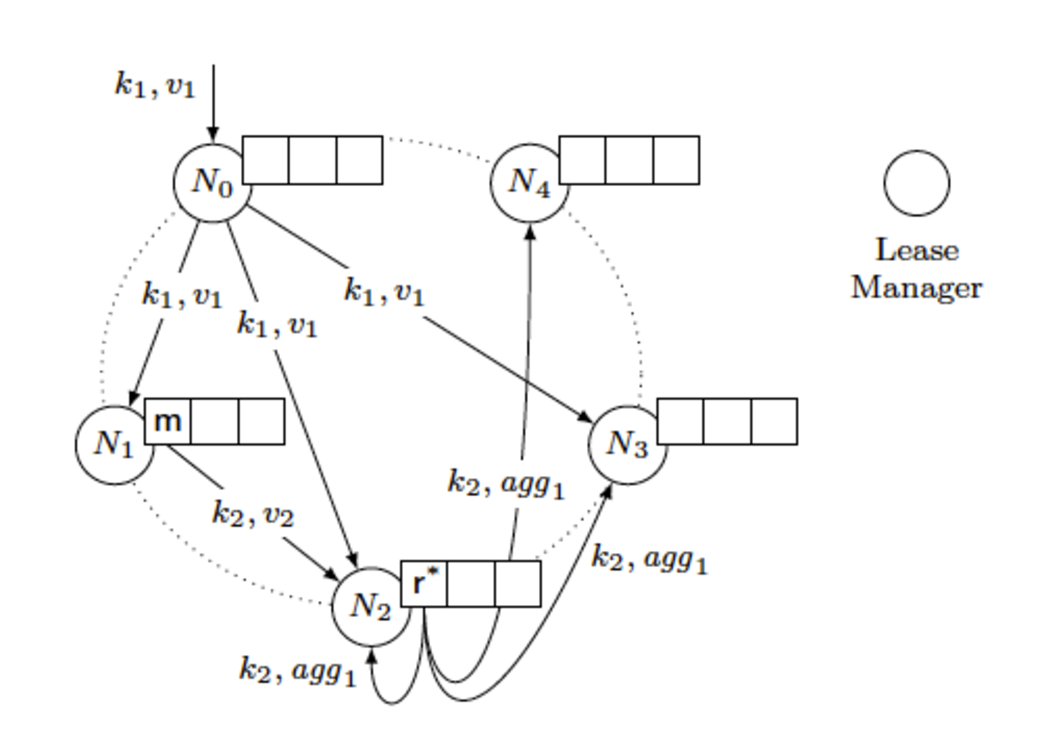
\includegraphics[width=4in]{../figures/realtimep.pdf}
\caption{实时MapReduce模型下map/reduce*的执行流程}
\label{fig:realtimep}
\end{figure}

图\ref{fig:realtimep}展示了一个如何利用本系统进行实时计算的流程。每当一个key-value对被插入到Cassandra系统中的时候,该节点就会执行一个分布式的事务:1)复制该key-value到多个节点;2)选择一个备份节点作为执行map程序的协调者;3)将map任务放入本地的任务队列中。而map任务的执行也是一个分布式的事务:1)将任务从队列中移除;2)将map输出写入到对应的reduce*节点;3)将reduce*任务放入到本地任务队列。而map输出将相同的key值路由到相同的节点中,reduce*的输出会将结果保存到多个节点中。事实上reduce*的执行过程也被视作一个分布式的事务,包括将数据写入多个节点中,以及将reduce*任务正确的从任务队列中移除。

\subsection{前人工作的不足及新的方案}

虽然上一节我们已经简单的介绍了很多分布式计算模型,然而实际上单纯列举已有的分布式计算模型就远远超过了本文的篇幅,我们在这里按照数据访问的模型对他们进行一个简单的分类并且分别讨论他们的缺点和不足。

上面我们所描述的编程模型中很大一部分是同步的数据流模型,这些模型针对的是那些面向数据流,并且对数据流进行同步的多轮处理的应用程序。比较典型的代表如MapReduce\cite{dean2008mapreduce}以及Dryad\cite{isard2007dryad}模型,以及一些基于它们的扩展模型\cite{bu2010haloop,ekanayake2010twister,zhang2011priter}。这些模型非常适合处理那些不需要访问全局共享状态的批处理应用,像\textit{wordcount}或者\textit{sorting}能够被很容易的在该模型下实现,这其中的一些扩展模型能够处理迭代计算,不过MapReduce模型本身的数据流模型使得访问计算中间状态变得非常复杂,这个限制使得这类编程模型在复杂的迭代计算场景下还是显得无能为力。

一些编程模型提供了面向数据的模型,比如Piccolo\cite{power2010piccolo}以及Pregel\cite{malewicz2010pregel},这些模型提供面向对象的数据访问语义,允许用户直接访问任意的数据而不须将数据抽象为数据流来处理。由于没有数据流的概念,为了保证并发执行时数据的一致,该类模型需要引入全局屏障(global barrier)以同步程序的执行。同步的计算模型抽象虽然简单,但是却会极大的提高程序的执行时间,因为每一个阶段的执行时间都是由最慢的执行所决定。

与同步面向数据的模型相对应的是提供了异步语义的面向数据的编程模型,比如Oolong\cite{mitchell2012oolong}以及GraphLab\cite{Low:2012:DGF:2212351.2212354}等,其中GraphLab是一个针对图应用设计的编程模型,用户需要将其需要解决的问题抽象成为图算法来解决,这在某种程度上也限制了其应用范围。

Oolong和Percolator同属于递增编程模型,它们针对递增处理应用而设计,从模型的角度来说很好的解决了递增计算和迭代计算对模型的需求,然而却在同步和错误处理上存在较大的问题。对于数据同步,Percolator选择使用分布式事务来管理程序执行的状态,Oolong则是通过用户提交的聚合函数作为全局屏障来同步程序的执行。Percolator的问题在于大量的事务和锁非常容易使得开发人员写出效率低下的分布式代码;而Oolong使用的聚合函数过于简单,对于稍微复杂的同步需求就无能为力,这类面向递增处理应用而设计的编程模型太过简单,并且非常有针对性,无法作为一种通用的编程模型出现。

面对这些编程模型的问题,我们提出了一种基于触发器的通用编程模型并且基于该模型设计和实现了运行时系统,统称为Domino计算模型。该模型特别适用与对时间要求较高的迭代和递增应用,亦可作为一种通用模型用于多种应用中。该计算模型具备以下几点创新性:

\begin{enumerate}
\item 完善了触发器的基本概念,在分布式环境下提出了将触发器作为通用的基本编程模型的思路和设计方案,能够用于不同的应用程序。

\item 提出了聚合模式对触发器的执行进行聚合,通过引入三种不同的同步模型:完全异步、最终同步、严格同步来支持同步及异步的应用。

\item 提出并实现了一种基于触发器的编程模型上的实时的容错恢复策略,能够有效的降低由于节点失效带来的应用处理速度延迟。
\end{enumerate}

一个典型的Domino的应用是通过组合一系列的触发器实现的。每一个触发器都是由用户编写的代码块组成,并且在特定的事件发生的时候被触发执行。比如在一个电子商务网站中,系统需要根据用户的购买历史和点击评分推荐其最感兴趣的商品,为每一个用户计算推荐商品的过程通常是若干个机器学习算法的组合。由于需要处理的数据量较大,且每一次完整的计算过程复杂度较高,因此通常需要在后台离线的计算,从而无法根据用户当前点击的情况为其推荐商品。然而用户当前的点击情况恰恰最精确和及时的反应了他的购买兴趣。然而使用触发器模型编写的推荐算法,可以通过监测用户点击事件来执行。执行过程中只需要对发生改变的部分数据进行重新计算,从而极大的降低了计算复杂度,能够实时的给出准确的推荐结果。

触发器模型虽然在此类在线复杂应用中效果较好,但是作为一种通用的编程模型却存在一些重要的挑战。这些挑战包括下列两点,我们在后面的Domino系统的设计和实现中将描述这两个挑战是如何在Domino中得到解决的。

\begin{enumerate}
\item 计算的同步问题。触发器模型的动作执行原生上是完全异步的,没有有效的同步控制方法,但是同步多个并行的计算流程却是分布式应用最基本的需求。比如MapReduce应用的Map和Reduce阶段直接天然的形成了同步语义,而MPI/OpenMP等应用中也需要用户显式的插入同步原语来保证不同执行语义的同步。

触发器模型无法简单的套用这类方法,原因如下。假设用户提交触发器$tr$以监测数据集$D_s$,当$D_s$中数据发生改变的时候,在不同服务器上的$tr$就会执行,并且产生需要同步聚合的中间结果。若该触发器程序处理的输入集是不断变化的(递增计算中较常见),那么系统在某一时刻有多少个$tr$会执行是是不可知的,该数目仅仅与当前输入数据集的改变有关。这也就导致我们无法在同步点准确的知道需要等待多少个$tr$的执行结果,因此无法有效的判断同步返回时刻。如果Domino应用不需要处理变化中的数据集,这个问题就可以通过使用传统的同步原语比较简单的解决。

\item 触发器模型将一个大规模的计算任务划分成针对数据改变的小的并发任务。这些并发任务的粒度较小,且并发的运行在大量的服务器中。这引入的一个大问题就是如何对节点的崩溃和任务的异常进行检测、恢复。

由于基于触发器模型的应用程序多需要处理不断流入的数据流并且较快的给出结果,如果触发器的某些节点上的实例由于节点失效而无法处理,就需要快速的恢复策略,而不能像MapReduce模型那样重新提交任务执行。为了支持实时的应用,须在触发器模型上实现更为有效的容错和恢复策略。

\end{enumerate}

\section{基于触发器的编程模型}
\label{section:intro}
\subsection{触发器模型}
触发器的概念在计算机科学中出现已经超过30年了,因为在很多传统系统中,组件需要对刚刚更新的对象进行识别并且针对性的执行一系列的操作。普遍认为这种方式能够提供更好的软件模块化能力,因为更新模块和处理该更新的模块可以独立起来。比如,一个雷达物体扫描程序会不断的更新敌军飞行器的位置,那么我们系统中应该同时有一个基于敌机出现或者位置改变发射火箭进行摧毁的模块来响应雷达扫描程序的输出。通常有两种做法来完成此类工作:一种是该模块不断的检查(\textit{轮询})感兴趣的对象,并且当发现对象发生改变时执行特定的动作。此方案最大的缺陷就是浪费资源,并且响应时间完全受限与轮询的时间间隔,而若设置较小的时间间隔,会浪费更多的资源。另外一种则是模块在某处等待直到感兴趣的对象发生改变才被激活执行特定的动作,我们也称之为触发模型。

从上个世纪90年代起,数据库领域出现了研究主动数据库(Active database\cite{rabuzin2007theory,mccarthy1989architecture, jaeger1999parallel, gehani1991ode,dayal1988hipac,chakravarthy1994composite})的热潮,主动数据库就核心概念就是利用触发器实现的一种面向数据的主动执行的概念。在主动数据库中,数据库操作或者外部的事件在满足一定条件的基础之下都能够触发特定动作执行。从概念上来说,主动数据库中的执行流程满足ECA规则,ECA即Event-Condition-Action。当一个事件发生的时候(On Event),并且特定的条件被满足了(IF CONDITION),然而指定的动作就将被执行(THEN ACTION)。主动数据库后来被广泛实现于商用数据库系统中(一般都是通过触发器或者触发器过程来实现),比如Postgres\cite{stonebraker1988postgres},HiPAC\cite{dayal1988hipac},Sybase\cite{darnovsky1987transact},VBase\cite{andrews1987combining}以及OOPS\cite{schlageter1988oops}等。然而直到今天,我们可以发现,虽然在理论上已经有很多关于ECA规则的研究,然而作为主动数据库理论核心的触发器依然是作为一个保持数据一致性、完整性或者安全检查的辅助工具存在于数据库中,没有成为通用的编程模型,其中主要原因是数据库由于需要支持ACID属性,使得触发器的实现复杂度太高:虽然相比较传统的面向程序的编程模型,基于触发器的编程模型能够在触发器数目较小的情况下提供明显的响应速度提升,并且通过将较大的应用分解成为一个个小的触发器来模块化应用并加以管理,不过,由于触发器对数据库领域最为核心的ACID特性,特别是事务机制的挑战,使得触发器的执行效率非常低。

不过情况在分布式环境下开始发生变化。根据之前介绍的CAP所描述,在一个分布式的系统无法同时提供一致性、可用性以及分割容忍三个特性。而且现有的云环境中,我们更加重视可用性和分割容忍性,因此一致性往往成为我们牺牲的选择。在新的NoSQL或者NewSQL的分布式存储系统中,人们尝试提供最终一致或者仅仅单节点内的原子性等。在这种情况下,分布式环境下,触发器模型也逐渐成为一个好的选择。

\subsection{Domino的编程模型}
Domino严格遵守了ECA模型,它将一个用户程序抽象为:事件监控(Event)、条件判断(Condition)、以及动作(Action)执行三个部分。为了更清楚的展示如何使用Domino模型来编写应用程序的,我们这里使用一个简单的分布式爬虫作为例子来介绍。

\begin{quotation}
\textbf{[分布式爬虫实例]}最基本的分布式网页爬虫非常简单,它开始于几个简单的网页URL地址,不断的将这些网页读取下来并且进行分析,通过分析网页的外链,爬虫将会获得更多的网页URL地址,周而复始直到爬取到某种限额或者整个网络。当然,一个可以工作的网络爬虫不止这么简单,它需要遵守Robots协议,需要考虑到网络带宽,需要考虑页面更新等等。而在我们的这个简单的例子中,我们并不会把重心放在这些功能上,而是更加关注网络爬虫的核心功能:爬取页面,分析页面。

本文实现的爬虫并不爬取互联网上的通用网站,而是爬取一个新型的社交网络上的信息(新浪微博)。微博是一种新型的社交媒体,所有的用户都可以发表公开的不超过140字的消息并且评论、转发他人的消息。由于其简单且交互性强而非常活跃。由于其时效性强,我们希望爬取能够爬取最新的消息,并且希望我们的爬虫可以以更高的优先级爬取那些\textit{更重要}的消息。这里的\textit{更重要}使用评论数加转发数的方式来定义,如果一个消息的评论数和转发数更多,那么它就更加重要。

基于Domino实现的网络爬虫程序的过程主要包括两部分,首先通过编写触发器监控存放微博信息的表,当用户有微博更新的时候,触发动作执行来获取该微博所有的评论或者转发的用户。这些用户我们称为\textit{当前活跃用户},并且记录下来。每次发现新的当前活跃用户,另外一个触发器就会执行,尝试抓取这些\textit{当前活跃用户}最近的微博消息,写入存放微博信息的表中,写入成功就会再次触发第一个触发器执行,以次往复,爬取微博消息。具体来说,触发器\textit{WBContentTrigger}负责监控微博消息表,当其中出现新的微博的时,获取该微博的所有评论或者转发的用户的信息,写入到微博用户信息表中;触发器\text{WBUserTrigger}负责监控微博用户信息表,当该表中某一个用户状态发生改变,意味着最近该用户曾经评论或者转发过别的用户信心的时候,该触发器将负责爬取这个用户最近的微博消息,并且写入到微博消息表中。
\end{quotation}

\subsubsection{事件(Event)}
触发器模型中,首要的元素就是ECA中的Event即事件。事件的种类非常多,按照之前在主动数据库中的分类,事件一般可以被划分为简单事件和复杂事件。其中简单事件主要包括了:时间事件(包括绝对时间事件和相对时间事件),方法事件(比如某个方法被调用而产生的事件),事务事件(比如事务提交或者准备事件),以及数据事件(比如数据被读取或者写入产生的事件)等。而复杂事件则是简单事件的组合或者是使用简单事件加上某些特定语义来组合,比如在某一个时间周期内未出现某个事件就被认为是一个复杂事件等等。然而在Domino中,我们主要关注的应用场景就是希望对存储在系统中的数据变化进行监控,因此我们主要提供了数据事件,特别是写数据事件的实现。当然时间事件也是很应用很广泛的事件源,不过由于分布式场景下时间的不一致导致我们无法给出一个用户一个统一的准确的时间线。由于时间的不统一,使得可用的时间事件粒度较粗,比如每个一个小时、每隔一天。对于这种应用,我们可以很简单的将时间事件委派给周期任务去执行,而不是通过Domino来实现。因此,Domino中主要关注了数据写事件。

\begin{figure}[h!]
\centering
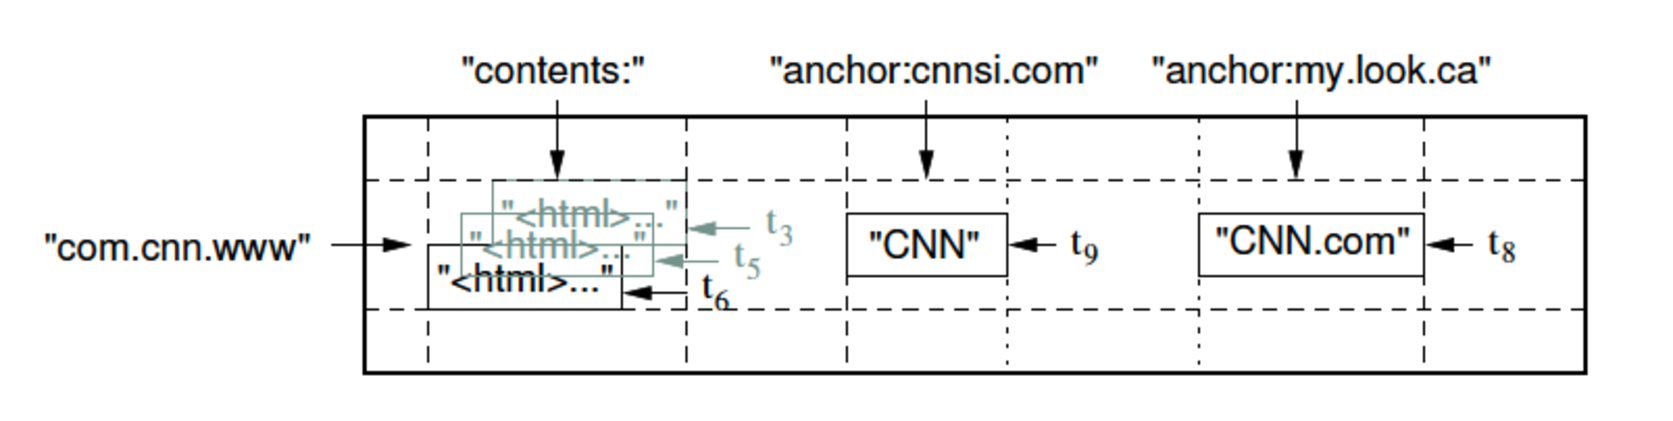
\includegraphics[width=4in]{../figures/bigtable.pdf}
\caption{HBase的基本数据单位:表的组成}
\label{fig:hbase}
\end{figure}

数据写事件来源于外界或者触发器本身对底层存储系统的写动作。当前版本的Domino是基于HBase实现的,因此我们首先对HBase中存储的数据结构进行一个简单的介绍。在HBase\cite{chang2008bigtable}中,数据是以表为单位存储的。表中的元素通过使用行关键字来区分,每一个行关键字都可以是任意一个字节串,而且HBase保证了所有针对字节串的读写都是原子的。如图\ref{fig:hbase}所示,HBase中的每一个表通常包含了数以亿行的数据,每一个行最多可以存储上千个列族以及上百万个列。列是以列族的方式组织起来的,每一个列族中可能包含不定数目的列,这些列可以在程序运行的过程中随时增加,列族也是进行访问控制的最小单元。每一个行列定位一个cell,其中存储着多个版本的数据。数据版本是一个64bit的整数。在cell中所有数据按照数据版本顺序以堆栈的方式堆叠起来。HBase中,如果想要使用某一个列族,开发人员必须事先新建该列族,或者通过改变表的属性来增加列族,列族被创建之后列才能被使用,用户通过指定\textit{列族:列}来制定一个cell。前面提到了Domino是通过修改HBase来实现的,在Domino中,我们要求用户提交触发器的时候指定所要监控的事件,默认情况下就是数据更新事件。这个事件中必须制定所监测的表、列族,列则是可选的,如果不指定列,那么所有该列族中的列上的更改都会产生数据更新事件。



\begin{table}[hb]\small
	\begin{minipage}[t]{0.5\linewidth}
	\centering
	\caption{HBase中表\textit{WBContent}的结构}
	\label{table:wbcontent}
	\begin{tabular}{|c|c|c|}
		\hline
		\textit{MessageId} & \textit{Content:zh} & ...,... \\
		\hline
		\textit{Message-1} & $content_{1}$ & ...,... \\
		\hline
		\textit{Message-2} & $content_{2}$ & ...,... \\
		\hline
		... & ... & ...\\
		\hline
	\end{tabular}
	\end{minipage}
	\begin{minipage}[t]{0.5\linewidth}
	\caption{HBase中表\textit{WBUser}的结构}
	\label{table:wbuser}
	\centering
		\begin{tabular}{|c|c|c|}
			\hline
			\textit{User Id} & \textit{Activity:recently} & ...,... \\
			\hline
			\textit{User-1} & $true$ & ...,... \\
			\hline
			\textit{User-2} & $true$ & ...,... \\
			\hline
			... & ... & ...,...\\
			\hline
		\end{tabular}
	\end{minipage}
\end{table}

\begin{quotation}
\textbf{[分布式爬虫实例]}在Domino网络爬虫的实现中,我们需要监控两个数据写事件。一个来自由于爬取到新的微博数据而修改的WBContent表的列: \textit{Content:zh},另一个来自于由于猜测到某些用户可能最近更新了微博页面的WBUser表的列:\textit{Activity:recently}. (触发器WBContentTrigger所监控的表如\ref{table:wbcontent}所示,而触发器WBUserTrigger所监控的表如\ref{table:wbuser}所示)。
\end{quotation}


\subsubsection{条件(Condition)}
触发器模型中,条件是一组用户自定义的函数。该函数的传入参数是封装好的事件,返回值为true或false来表明当前用户制定的条件是否满足。在Domino中,条件(condition)包括了三种,分别负责三个关键的功能:首先,由于触发器一旦提交到系统中就会持久存在除非用户显式的取消该,但是在大多数情况下,我们希望触发器能够在到达某些条件的时候自动停止,而不是永远运行。在这种情况下,用户就可以通过编写停止条件(stop condition)来实现判断。除此之外,由于Domino中的事件都是由数据写入引起的,如果短期内写入频率非常高,对它们进行快速处理就会极大的占据系统资源,在这种情况下,用户就可以通过编写间隔条件(interval condition)来为每一个触发器指定执行的周期。其实在Domino中,每一个活跃的触发器都是有一个最大执行频率的,用户可以通过编写条件函数覆盖该设置以加入自己的频率控制语句。最后,Domino还引入了选择条件(select condition)来对事件进行选择,仅仅处理其中一部分事件,该条件对于很多高效应用非常重要。

停止条件(stop condition)中非常的应用在那些迭代收敛的应用中。比如PageRank或者很多机器学习算法,这些算法中,往往需要判断连续两次迭代中计算的值之差是否足够小。如果足够小,程序就可以停止运行。Domino对这种应用做了特别的优化,每一个传入条件函数的封装好的事件都包括了更新前的值和更新后的值。

\begin{quotation}
\textbf{[分布式爬虫实例]}对于爬虫来说,我们不需要特别的停止语句,因此我们将默认使用Domino本身提供的条件函数(如\ref{code:wbcrawler}的filter函数所示),实际Java代码实例如下:
\begin{lstlisting}[language=java]
  //过滤器,用来判断这个事件是否应该使触发器执行。这里永远返回true
  @Override
  public boolean filter(HTriggerEvent hte) {
    return true;
  }
\end{lstlisting}
\end{quotation}

\subsubsection{动作(Action)}
触发器模型中,动作函数(Action)是由用户编写的一段代码块来执行所需要的代码逻辑。Domino为用户的动作函数提供了完整的变量封装以提高用户代码执行的效率,如\ref{code:wbcrawler}中的HTriggerEvent对象。在该对象中,Domino为用户程序封装了多个相关值供其操作,这些值包括:触发该事件的数据更新动作相关的行关键字的值;该触发器所监测的列族或者列中数据的新值以及更新操作之前的旧值;事件发生的时间和上次同样的事件发生的时间。除此之外,我们还封装了相关的环境变量。比如触发器执行时所在节点的信息以及某些用户提交触发器时显式设置的变量及其值。

Domino为用户提供的是面向数据的编程模型,其允许用户在动作函数中任意访问需要的数据并且加以修改,并不需要像MapReduce或者Storm模型那样,必须按照数据流来组织应用和访问数据。这种方式简化了用户代码,不过也带来了问题。首当其冲的就是效率问题,允许用户在高频执行的动作函数对分布式存储系统(HBase)中的数据任意读写,特别是写,将给存储系统带来极大的压力,并且也会严重影响动作的执行速度。因此我们为这种情况专门提供了延迟写的异步语义,用户在动作函数中对分布式存储系统的写操作会被缓冲在本地的WritePrepared实例中,直到该动作函数退出前统一调用flush函数实施真正的写入操作。这一部分详细内容我们将在第\ref{section:io}部分进一步详述。

\begin{quotation}
\textbf{[分布式爬虫实例]}本应用中动作函数非常简单:对任意一条消息,找到所有曾经评论或者转发它的用户,并且将该用户的数据写入到WBUser表中。对每一个用户,爬取所有其最近发表的所有消息,并且存储到WBContent表中。具体的Java代码参见\ref{code:wbcrawler}中两个触发器中的action函数,或下面的代码节选。
\begin{lstlisting}[language=java]
  @Override
  public void action(HTriggerEvent hte) {
    byte[] msgId = hte.getRowKey();
    byte[] msgContent = hte.getNewValue();
    String msgContentStr = new String(msgContent);

    ArrayList<String> aus = this.getUsersByAPI(new String(msgId));
    for (String userId : aus){
      Put p = new Put(userId.getBytes());
      p.add("Activity".getBytes(), "recently".getBytes(),
      		  "true".getBytes());
      this.writer.append(p);
    }
    this.writer.flush();
  }
  
  @Override
  public void action(HTriggerEvent hte) {
	byte[] userId = hte.getRowKey();
	Timeline tl = new Timeline();
	tl.client.setToken(this.accessToken);
	StatusWapper status = tl.getUserTimelineByUid(new String(userId));
	for (Status s:status.getStatuses()){
		Put p = new Put(msgId);
		p.add("Content".getBytes(), "zh".getBytes(), s.getText().getBytes());
		writer.append(p);
	}
	this.writer.flush();
  }
\end{lstlisting}
\end{quotation}

Domino模型在动作函数中一个关键的不同于现有的基于事件的分布式计算模型(比如Percolator或者Oolong)的地方:如何实现聚合操作。分布式爬虫的实例中不存在聚合操作,为了说明聚合操作的作用和重要性,我们这里简单的扩展该爬虫:当从某消息中获得所有曾经评论或者转发它的用户后,且将这些用户数据写入到WBUser表之前,出于某种原因,我们需要判断该用户所评论或转发的字数之和是否超过一定阈值,如果超过才认为他是活跃的并且写入到WBUser表以进行爬取工作。实现该功能,就需要搜集到所有同关键字的数据,并且加以聚合,就需要使用到聚合操作。

在Oolong这样的事件处理系统中,用户可以使用一系列显式的,事先定义好的聚合函数,比如求和、最大(小)值等。不过这些函数都太过简单,限制了实现很多复杂的逻辑的可能性。Google的Percolator完全没有对聚合操作提供额外的支持,所有的聚合动作都由用户通过使用事务机制自己实现(通常通过加分布式锁来实现),这对于不熟悉分布式系统的开发人员来说并不是一个好的选择。不同于已有系统,Domino设计了一个专用与聚合操作的设计模式:聚合模式。当用户需要聚合操作的时候,他可以完全按照聚合模式的指导来设计系统:首先,与原有触发器一起提交一个聚合触发器;其次,对所有需要聚合的触发器,修改其WritePrepared实例,引导结果写入到刚才提交的聚合触发器而不是HBase的表中;最后,通过修改聚合触发器中的动作函数来完成用户逻辑。通过这种方式,所有需要聚合的中间结果将被写入到一个隐式的表中($t_{acc}$),聚合触发器会自动检测该表上的变化,并且运行用户提交的动作函数。

引入聚合模式仅仅是解决了如何将来自不同的触发器动作产生的结果结合在一起的问题,紧接着的问题就是什么时候执行聚合模式中的动作函数:当来自不同服务器的触发器动作试图更新($t_{acc}$)中的数据时,它们往往是不同步的。然而,编程框架无法判断是否应该在触发器动作处进行同步等待或者可以异步向下执行,这跟应用程序有很大的相关性,因此Domino为不同的应用类型提供了不同的同步模型。


\subsection{同步模型}
\label{section:sync}
这里所说的同步和异步不同于I/O系统中的同步、异步,而是指多个并发执行流之间的同步。在分布式程序的执行过程中,如果当前计算需要聚合多个并发运行的子任务产生的数据的时候,就需要对这些子任务进行同步操作。同步模型意味着计算的继续需要所有子任务的结果都已经产生;而异步模型意味着计算只需要发现有子任务产生结果就可以继续运行。

\subsubsection{严格同步}

同步模型下运行的程序往往会带来很大的性能损失,这也很容易理解,因为程序的执行需要等待多个分布式子任务中最慢的那个完成才能继续,不过由于很多程序或者算法本身必须遵循该模型才能得到正确的结果,因此Domino中对该类应用提供了严格同步的原语以帮助实现这些算法。

假设一个触发器在多个服务器上独立运行,并且在某一个节点需要一个严格同步的场景,在Domino中可以简单的通过使用同步模式来实现:在节点处实现一个聚合触发器,该触发器所配备的表会存储所有需要同步的中间计算结果。此时问题的关键就在于聚合触发器上的用户动作什么时候开始执行,它是如何知道所有需要同步的任务都已经执行到同步点了呢?

在Domino实现中,我们提供了两个原语($register$和$waitSync$)来提供严格同步的功能。首先所有需要进行同步的触发器动作刚开始执行的时候都需要先调用$register$来注册自己,每次注册成功后会在ZooKeeper中生成一个临时节点,节点的名字为\textit{triggger-id}加当前执行序列\textit{id},该节点中会存储一个count值,每次动作在注册的时候将count值加1。当触发器动作执行完退出的时候会将ZooKeeper中对应的节点中的值减1,如果减一后节点值为0,那么就删除该节点。所有调用$waitSync$的动作函数都根据当前执行序列id,挂在ZooKeeper的对应节点上同步等待。当节点被删除的时候,$waitSync$返回,开始执行用户逻辑。此时可以保证所有需要同步的节点上的触发器动作都已经执行完毕了。


\subsubsection{完全异步}

与同步模型相比,异步模型是另外一个极端,它永远以分布式子任务中最快的那个为标准执行,从而具有更好的执行速率,并且很多算法都被证明异步结果和同步结果非常接近,并不会影响到结果的正确性。比如很多线性\cite{bertsekas1989parallel}的数据挖掘和机器学习算法(belief propagation\cite{gonzalez2009residual}, expectation maximization\cite{neal1998view}, stochastic optimization\cite{macready1996criticality, smola2010architecture}, 以及PageRank等)。Domino本身的触发器语义天然的支持了这种全异步的模型:触发器被自动的指派到不同的节点上独立执行,并且触发器之间没有隐式的同步动作。

\subsubsection{最终同步}

为了平衡同步应用对性能的要求,Domino除了提供同步异步模型外,还设计了一套最终同步的模型,专门用来提高那些需要较好的响应时间,且不能够简单改写为异步模型应用的性能。

\begin{figure*}[h!]
\centering
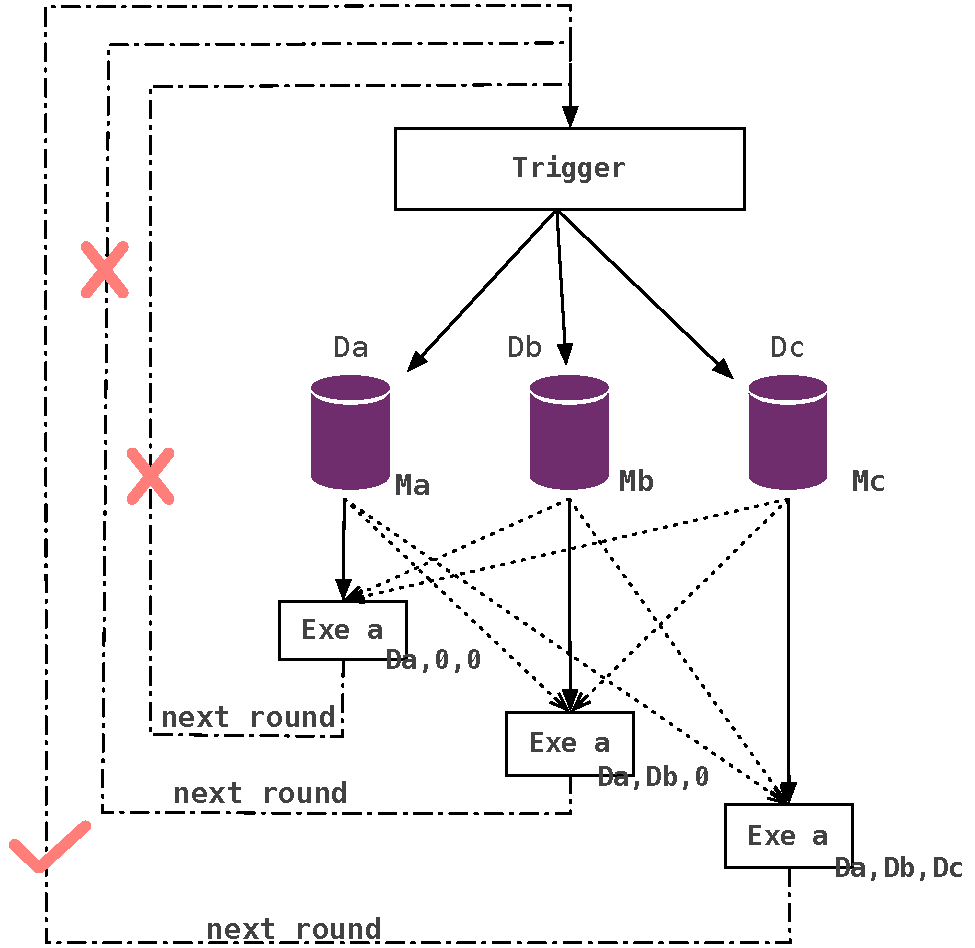
\includegraphics[width=5in]{../figures/sync.pdf}
\caption{最终同步的基本概念}
\label{fig:sync}
\end{figure*}

最终同步模型中,程序的执行不需要等待所有的子任务都完成,程序可以提前向下执行,但是在足够的时间窗口后,最终还是会得到同步执行相同的结果。图\ref{fig:sync}列举了在三台服务器($Ma, Mb, Mc$)上执行的三个触发器动作需要进行聚合时的情况,聚合$Da, Db, Dc$三个值。服务器$Ma$上的触发器首先计算出$Da$,此时$Mb$和$Mc$都没有完成计算,此时计算不会等待,而是根据$Da, 0, 0$计算出结果(这里的0不是指值为零,而是数据版本号为0,可参考下面的描述);随后$Mb$和$Mc$先后完成计算,产生了$Da, Db, 0$和$Da, Db, Dc$两个值。最后触发的$Mc$产生的值会覆盖掉之前的部分值,作为最终同步的结果出现。

Domino中最终同步模型基于HBase的多版本表实现,它可以用于同步两个不同的触发器,也可以用于上一节我们描述的聚合模式。比如,当用户需要聚合操作,并且需要在聚合操作处进行同步的时候,只要伴随需要聚合的触发器再提交一个聚合触发器即可。系统会自动创建一个仅本应用可以访问的隐式表,该表存储的所有数据都是带有版本信息的。表中任一个cell上数据的版本信息等于将该数据写入表的触发器动作的执行序列id,而触发器动作的执行序列id则是从0开始,每次执行自动加1的。聚合触发器的动作(Action)则根据表上的数据更新操作来执行:每次数据更新都会触发动作执行用户定义的聚合操作,那么这个动作的执行序列id就是更新后的数据的版本号。执行聚合操作需要读入表的数据,Domino模型确保该函数只能读到小于或等于当前执行序列id的数据,最终产生的结果的版本id也是当前动作的执行序列id加1。

\begin{figure*}[h!]
\centering
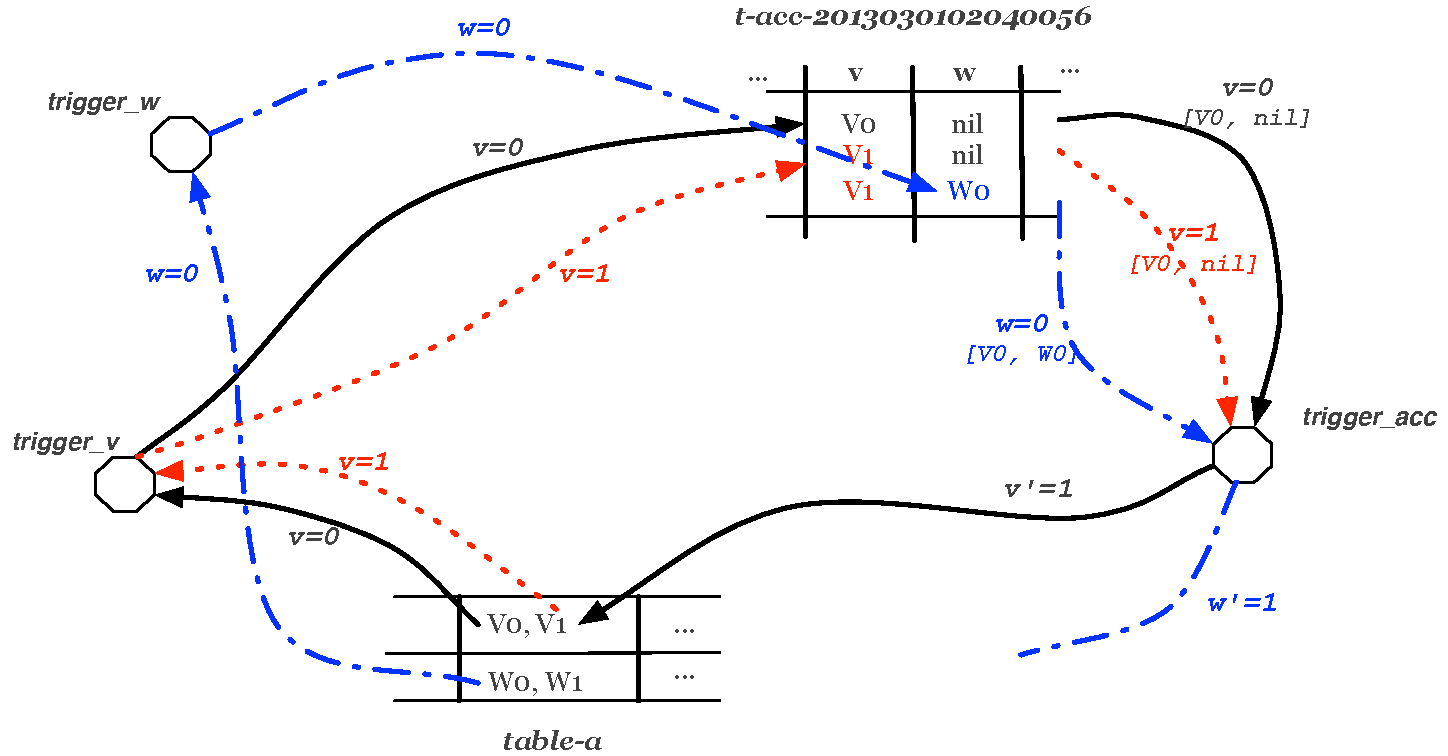
\includegraphics[width=5.5in]{../figures/multiv.pdf}
\caption{Domino中最终同步模型下多版本执行的流程图}
\label{fig:multiv}
\end{figure*}


图\ref{fig:multiv}展示了这样一个最终同步模型下多版本执行的流程。我们使用了两个触发器:$trigger_{[w|k]}$和$trigger_{acc}$来做示例。其中$triger_{[w|k]}$由表$table_a$触发,而$trigger_{acc}$用来帮助同步所有$trigger_{[w|k]}$实例产生的中间结果。表名字为t-acc-2013030102040056,由Domino系统自动创建,且仅在$trigger_{acc}$中可以访问。由图中可以看出$trigger_w$比$trigger_v$慢一些,当$v$已经运行到执行序列为1的时候,$w$刚刚开始它第0轮运行。那么在整个执行过程中,两个中间结果会被聚合触发器的动作函数根据输入$[v_0, nil], [v_1, nil]$计算出来并且写入到HBase的表中。这些结果未必正确,但是它能够作为中间结果被访问和使用。如果我们的算法中这些部分结果是有意义的,那么这些部分结果就能够被最早的加以利用,而不是所有的节点都等待最慢节点的执行。当然,随着$w$的执行,其最终也会将结果写入到表中,聚合函数根据版本顺序,取到的输入正好是所有同版本的数据,从而得到正确的结果。

最终同步相比较严格同步来说,不会发生停止等待的情况,不需要分布式锁的参与。特别对于那些中间结果有意义的算法具有非常好的效果,且其本身也可以保证最终结果与同步模型结果完全相同。因此在实际应用中有很多优势。不过其问题也非常明显,其中最大的就是资源浪费问题,如果大量的中间结果是无意义的,那么浪费计算资源去计算它们就没有意义。因此对于这类算法,还是应当采用严格同步的模型。

由于在最终同步的实现中,所有的序列id都是本地维护的,这样就存在一种可能性:具有相同执行序列的动作函数都试图向同一个位置发起写操作。在这种情况下,我们需要对这些写操作指定一个顺序来保证结果的正确性。在Domino中,我们定义一个触发器的某个动作函数的写序向量如下:
\begin{equation}
V^{T} = (V_{tc_{fired}}: V_{tc_1} : V_{tc_2}: ... V_{tc_i})
\end{equation}
其中等式右边的$V_{tc_{fired}}$代表触发该触发器动作执行的数据版本号,而$V_{tc_i}$则代表了触发器动作执行时访问的数据的版本号。当两个具有相同的触发器动作执行序列号的动作($i$和$j$)试图向同一个位置写入数据的时候,系统将比较他们的写序向量:首先比较$V_{tc_{fired}}^i$ 和 $V_{tc_{fired}}^j$,较大的动作写入;若相等,那么从前向后依次比较$V_{tc_i}$,同样是较大的动作写入。

通过这种方式设计的写顺序,通过简单的分析就可以知道:任何时候,一个全部到达同步点的写入带来的触发器动作一定比所有未完全到达同步点的触发器动作的写序向量大,这样就保证了最终同步的结果不会被覆盖。

\section{设计和实现}
\label{section:design}
本节中我们将介绍Domino运行时系统的实现以及其主要挑战的解决方法。我们将Domino系统设计成为使用Java实现的基于HBase的计算模型,并且和HBase以一种插件的方式一起运行,然而事实上Domino的实现并不限制与HBase,它可以与任何的分布式存储系统一起工作,只要存储系统提供持久性支持并且允许存储多版本的数据。我们现在正在将Domino移植到Sedna系统中。


\begin{figure}[h!]
\centering
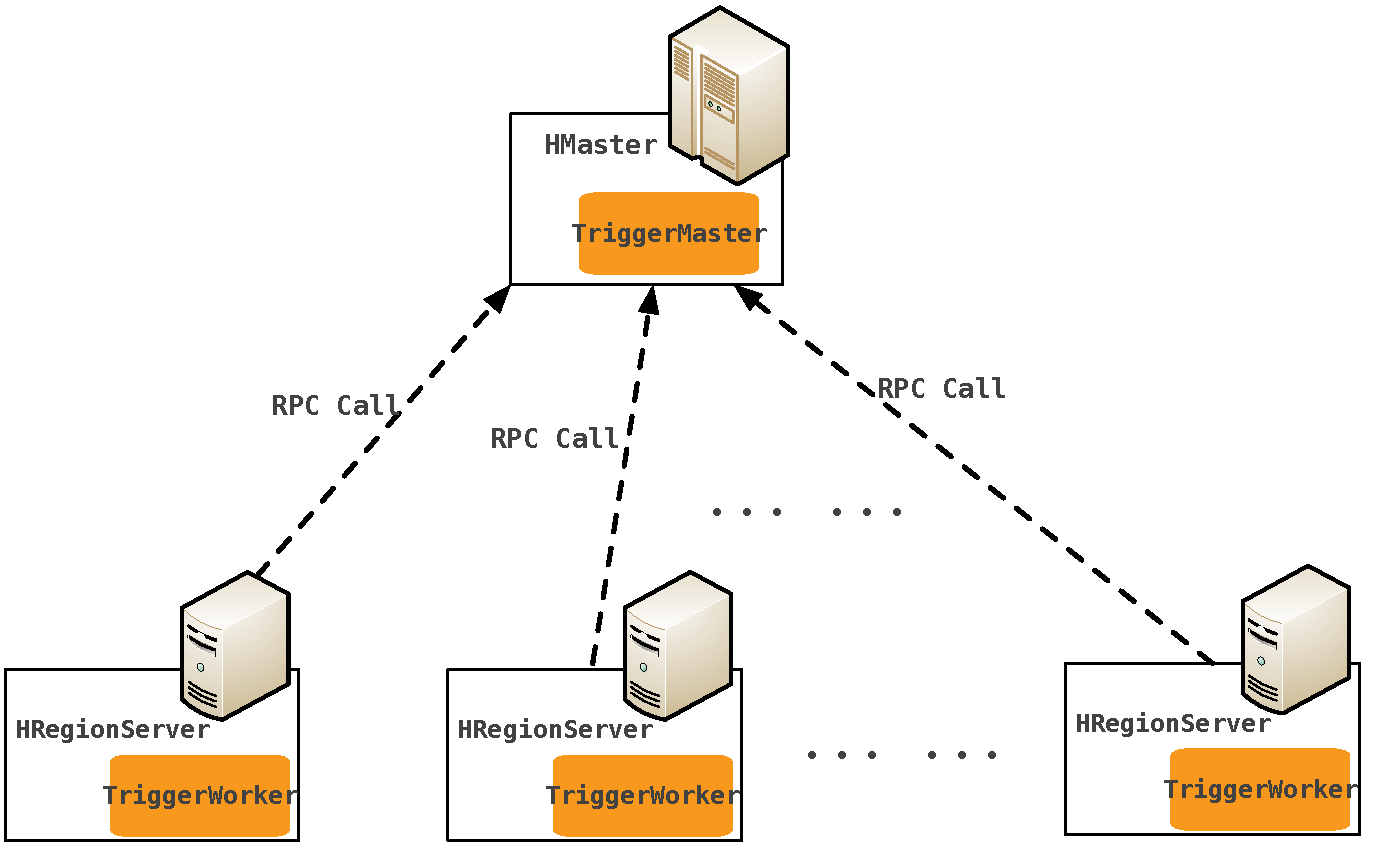
\includegraphics[width=5in]{arch1.pdf}
\caption{运行在HBase集群上的Domino集群的架构图}
\label{fig:arch1}
\end{figure}

\begin{figure}[h!]
\centering
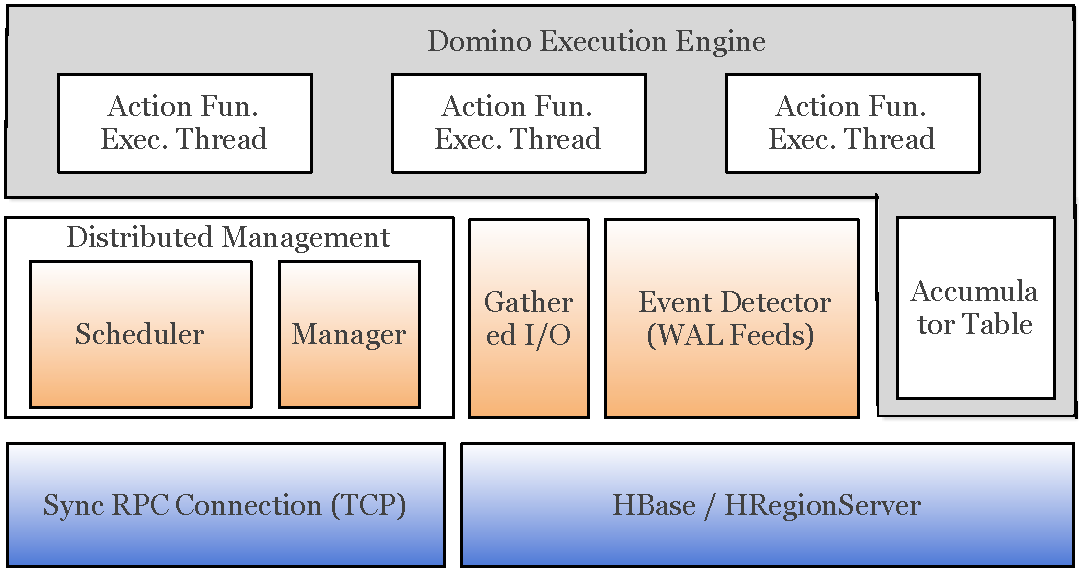
\includegraphics[width=5in]{../figures/arch.pdf}
\caption{Domino运行时系统的模块图,每一个模块都依赖于其下面模块提供的服务}
\label{fig:arch}
\end{figure}

图\ref{fig:arch1}和\ref{fig:arch}分别展示了Domino的系统架构以及不同逻辑模块之间的逻辑架构。Domino本身是基于HBase实现的,因此在实际运行中其节点之间的架构和HBase一致,都是由Master节点和Slave节点组成。HBase中的Master节点称为$HMaster$,slave节点也就是实际的Region存储的节点被称为$HRegionServer$;于此对应的是Domino的节点,Domino的Master节点$TriggerMaster$与HBase的$HMaster$运行在同一个物理节点上,而任务执行节点$TriggerWorker$运行在$HRegionServer$的节点上。所有的节点都运行着图\ref{fig:arch}中的各个组件,唯一的区别是$TriggerMaster$会运行其中的分布式管理(distribted management)部分,而$TriggerWorker$则不会运行这部分。不同的$TriggerWorker$之间通过同步的RCP远程调用来互相通信,而所有的$TriggerWorker$也需要和$TriggerMaster$保持一个心跳连接以汇报所有触发器的执行状态。需要注意的是,Domino的$HMaster$不是由用户手工指定的,而是在Domino启动的时候首次将自己注册成为$TriggerMaster$的节点充当。因此在Domino中不存在单点故障或者单点性能瓶颈。

\subsection{执行流程}
用户想Domino系统提交触发器采用MapReduce任务提交类似的方式:首先将需要执行的触发器相关代码打包成jar包,然后通过domino命令行程序提交到系统中去。下面的代码块展示了如何将上文中实现的分布式触发器提交给Domino的命令。其中WBCrawler为一个包含了main入口的主类,其负责提交另外WBContentTrigger和WBUserTrigger。
\begin{lstlisting}[language=bash]
	bin/domino trigger WBCrawler.jar wbcrawler.WBCrawler
\end{lstlisting}

用户向Domino提交触发器是通过新建并初始化一个Trigger对象,之后调用其submit方法实现的。下面的代码块展示了分布式爬虫实现中一个触发器(WBUserTrigger)的提交代码。用户需要新建一个Trigger对象,这个对象中必须设置触发器的名字,指定所监测的表、列族信息。如果这个触发器的检测对象具体到列族中的某个列,那么还需要调用配套的设置函数来设置,最后最重要的是需要设置该触发器触发时执行的类。这个类中应当包括用户实现的条件函数和动作函数。

\begin{lstlisting}[language=java]
Trigger tg2 = new Trigger("WBUserTrigger", "WBUser", "Activity");
tg2.setTriggerOnColumn("recently");
tg2.setActionClassName("wbcrawler.WBUserTrigger");
tg2.submit();
\end{lstlisting}

调用Trigger对象的submit函数后,Domino会首先从$TriggerMaster$处获得一个全局唯一的触发器id,之后将用户提交的jar包提交到HDFS存储系统由该触发器id组成的目录中。之后所有的$TriggerWorker$都将HDFS的该位置下载并加载需要的类。Domino会首先向$TriggerMaster$提交触发器。提交成功之后,会询问HBase的.META.表来获取本触发器所监测的表所在的$RegionServer$的位置。之后会依次向这些$RegionServer$提交触发器请求。只有所有的触发器请求都成功之后,提交才会返回。如果其中出错,Domino会负责回滚之前的操作,并且返回用户提交失败的信息。

触发器提交成功之后就已经开始在$RegionServer$处开始运行。此后,Domino在每一台服务器上都运行着事件感知组件(\ref{subsection:feed})负责监控数据更改,当遇到对象的数据修改的时候,用户提交的触发器代码就会被加载执行。触发器会因为停止条件(stop condition)而停止,也可以由用户提交命令显示的停止。在Domino中,用户程序可以使用Trigger对象的stop()方法来卸载一个触发器,也可以使用shell命令来完成:
\begin{lstlisting}[language=bash]
	bin/domino stop_trigger trigger-id
\end{lstlisting}
命令提交后,Domino会首先根据用户提交的‘trigger-id’来查找对应的trigger实例。如果存在,就会先卸载运行在$TriggerWorker$上的实例,所有实例卸载完成之后再卸载$TriggerMaster$上的实例,完成后返回。

\subsection{事件感知组件(Event Detector)}
\label{subsection:feed}
Domino的事件感知组件包括两部分。第一部分(WAL Feeds)作为主要的事件感知源用于在正常情况下对数据修改进行快速的感知;而另外一部分(Sequential Scan)则作为持久化事件的组件存在,当系统中出现错误的时候,该部分则保证所有未处理的事件都不会丢失。

\subsubsection{WAL Feeds}

HBase是一个保证了数据持久存储的分布式存储系统,它不会因为少量节点的故障而丢失数据。这是因为其会将所有的数据都存储在磁盘中,而磁盘则利用HDFS提供的多备份来保证数据的安全性。然而由于磁盘的响应时间过慢,为了提高IO性能,HBase会将所有的数据暂时存储在内存中,同时持久化在HDFS的WAL(write-ahead-log)中。为了保证数据不会因为在写操作的过程中节点突然崩溃而丢失,HBase会先将数据写入到WAL中,并且在写入成功后才开始将数据写入到内存中。写入到WAL中的数据是按照其在内存中的结构组织来写,而是将每一条数据整理成包括:行关键字、列族、列、值、时间戳、类型的日志,以顺序的方式写入WAL文件中,以提高磁盘I/O性能。

Domino的事件感知组件利用了HBase存储数据的特点,在每一个$TriggerWorker$中,Domino的事件感知组件都会将自己注册到HBase写入WAL文件的关键路径中,完全异步地对当前写入的日志数据进行判断,判断是否属于某个已注册的触发器所监测的范围。

\begin{figure}[]
\centering
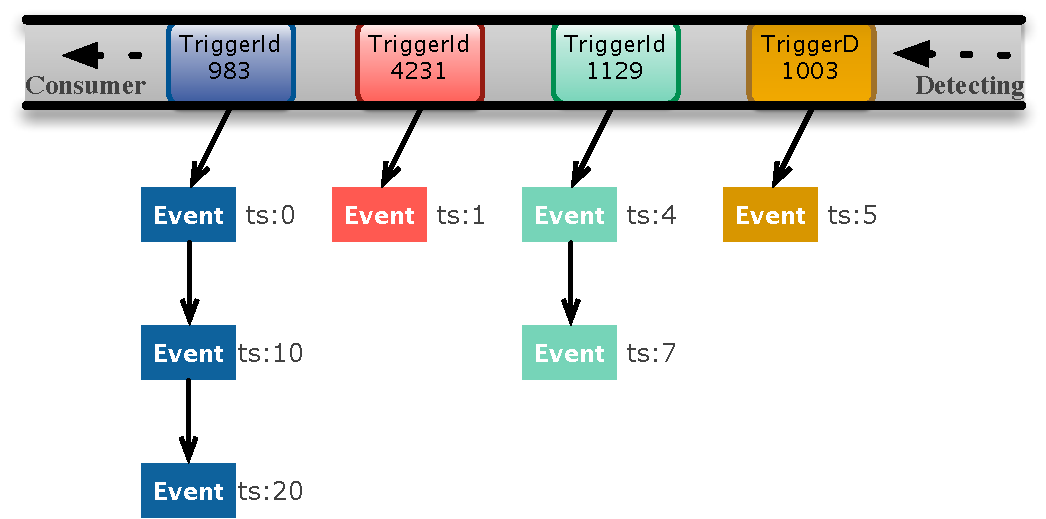
\includegraphics[width=5in]{../figures/queue.pdf}
\caption{Domino事件队列。如果两个事件属于同一个触发器,它们会整合被放入到队列中的同一个位置。队列中的顺序基于时间戳。消费者每次队列中取出属于同一个触发器的所有事件以减少频繁的进行线程切换带来的性能损失。}
\label{figs:queue}
\end{figure}

一旦事件感知组件探测到了一个对WAL文件的修改,并且该修改正好属于某一个已经注册的触发器的监测范围,它将封装一个包括了更新后的值以及更新前的值的事件(HTriggerEvent)并且将封装好的事件对象放入到事件队列中(如图\ref{figs:queue})所示。队列上有一个消费者不断的从队列中取出最新的事件来处理。最终,触发的事件会被发送到用户所写的条件函数和动作函数来处理。为了进一步提高效率,我们在每一个$TriggerWorker$中预先开辟了一个线程池,且为每一个触发器启动了一个线程,并且空置等待着事件到来执行。在实际的实现中,我们扩展了Java的同步线程库,使得所有的线程都变得可管理。具体表现在所有的子线程都有自动的异常处理、执行状态记录、重启等功能。

\subsubsection{顺序扫描}
WAL Feeds 组件对事件相应时间较低,适合作为主要的事件感知组件在Domino中运行。然而由于它的核心组件——事件队列是一直存在与单节点的内存中的,如果节点出现故障就无法恢复。这对于一个会长时间运行的分布式运行时系统来说是不可以接受的。为了在保证事件感知效率的前提下提高系统容错的能力,我们引入了Sequential Scan的策略来为Domino提供错误情况下的事件探测工作。

首先,由于Domino允许最小的监测单元是列,而HBase本身是将表按照列族分为独立的单元来管理的,因此同一行且同一个列族的数据一定在同一台服务器上存储着。我们修改HBase代码,为每一个列族默认的增加一列(\_events\_),每次HBase在向某一列族中的某一列写入数据的时候,系统会同时在\_events\_列中存储此次写入的本地唯一id,这个本地唯一id也会被存储到$HTriggerEvent$对象中,传给动作函数。用这样的方式,在WAL文件中,就会生成连续的两条写入日志:数据列写入和\_events\_列写入。另外一方面,当用户提交的触发器动作函数执行完毕的时候,Domino会自动将id从\_events\_列中删除。

如果Domino在运行过程中,某个节点崩溃,那么我们在WAL Feeds中所构造的事
件队列全部丢失,此时触发器会在另外一个节点上重新启动,而所有的崩溃节点
的数据也会在另外一个节点上由WAL文件进行恢复。在恢复的过程中,我们可以首先获得每一行数据,每一个列族的\_event\_列最新数据。上面记录了在事件队列中丢失了的所有的写入时的id。对每一个id,从后向前,逆着事件顺序搜索,当发现带有该id的WAL日志的时候,其前面那一条日志中存储的数据就是导致事件发生的,更新的数据的值。Domino会强制重新产生这个事件,进而继续之前未能执行的触发器动作。


\subsection{延迟写组件(Gathered I/O)}
\label{section:io}
Domino为用户提供了面向数据的编程模型,它允许用户在自己编写的函数中自由
的访问数据。但是这种模型也会带来很多问题。首当其冲的就是性能问题,因为
访问非本地数据是非常耗时的,而用户写的函数中可能多次调用这样的写操作从
而使得情况更加糟糕。另外一个问题就是数据的一致性问题,前面在介绍最终同
步的时候,我们介绍了如何解决同一个触发器不同的动作之间写冲突时一致性的
方案,而这里需要考虑的是不同触发器的写冲突。首先,对于单个写操作,在
Domino中,我们始终保证后写成功。在这个前提下,我们面临一个更复杂的情况:
由于我们允许用户自由的读写数据,那么有可能发生不同的触发器动作会进行交
错的写操作。比如触发器A写入$loc_1$,且成功,之后开始写$loc_2$;而触发
器B先写入$loc_2$成功后写入$loc_1$,这样最后结果是$loc_1$被A写入,
$loc_2$被B写入,任何一个触发器内部都无法得到一个一致的状态。

为了解决这些问题,在Domino中,我们提供了一个延迟写组件(WritePrepared)
帮助提高写效率,同时帮助在一个触发器内部维持一个一致的数据状态。
WritePrepared封装所有在触发器动作函数中发起的对HBase表格的写操作,并且
通过在一次动作函数执行完毕的时候调用flush方法来一次性的将WritePrepared
中缓存的数据真正写入到HBase的表格中。

WritePrepared中的缓存数据写入HBase表时是有序的,顺序是由调用flush操作
的时候从ZooKeeper获得的全局序列id($G_{id}$)决定的。当两个具有不同全局
id的写操作从Domino的触发器中发出的时候,如果两者并没有冲突(即没有写入
同一个位置),那么HBase并不会感受到有什么不同;然而如果两者产生冲突,那
么具有较大的全局序列id的写操作会被挂起直到前一个写操作完成。在挂起期间,
所有之前部分写成功的数据都会被冲突的那个、具有较小的全局序列id的写操作
覆盖。WritePrepared的flush顺序并不意味着我们将所有的分布式写操作都强制
排序了。强制对所有写操作排序会极大的降低写性能,我们只是通过版本控制保
证具有较低的全局id的flush操作开始后,它就不会被别的触发器抢占。

使用WritePrepared和flush操作,我们可以为触发器中的动作函数提供较高的
I/O效率,并且保证所有的写操作不会互相交错。

\subsection{容错和恢复组件}
容错能力是云计算平台下的计算模型面临的的最大的挑战。很多流式计算模型,
像Storm和S4这样的系统虽然具有较好的性能,但是其在容错和恢复上的短板同
样极大的限制了其应用。然而,Domino由于采用了基于触发器的模型,所有的中
间数据都可以保存在持久存储的分布式存储环境中使得我们能够有机会提供较好的容错能力以及错误恢复能力。

首先,Domino的各个组件通过HBase提供的容错能力作为其静态容错的基础:所
有提交的触发器信息都存储在HBase中,所有中间数据都被保存在HBase表中,触
发器的执行状态也通过序列id区别保存,聚合模式中自动创建的分布式表
($t_{acc}$)也持久存储在HBase中。这些信息都不会因为节点的意外崩溃而丢失。

除了静态容错外,由于触发器在Domino系统中时刻处于运行的状态,我们希望能
够对执行中的状态实现容错和恢复。比如正在执行的触发器所在的节点崩溃,或
者触发器本身线程崩溃,我们希望能够尽快的在备份节点上继续之前正在进行的
计算。

Domino节点中比较极端的情况是物理节点崩溃,这也意味着其上面运行的HBase
服务也离线。那么节点崩溃之后的所有更新操作都会被重定向到自动选出的备份
节点,并且在备份节点上会开始根据WAL中的数据重建内存数据结构。在备份节点恢复数据的同时,Domino的触发器会随之重新在备份节点上初始化并且开始运
行。这意味着,所有在节点崩溃之后新的数据写入操作都会如同没有发生错误一
样在新的节点上被触发器监测并且处理。

对于那些崩溃发生时正在执行的动作函数来说,所有能影响到HBase的输出都被缓存在WritePrepared中。若崩溃时尚未执行到flush,那么该动作函数的本次执行未完成,Domino在备份节点上重新运行该动作函数即可(只读入对应该执行序列id的输入数据);若崩溃时已经开始执行flush,那么这次动作函数的执行其实已经完成,只剩下最后的IO操作。为了能够保证完成所有的缓存在WritePrepared中的IO操作,在Domino中,除了前面所讲每一个的WritePrepared都在ZooKeeper中申请全局唯一序列号($G_{id}$)
外,我们还为每一个WritePrepared实例都在ZooKeeper上映射了一个临时节点,
其中存放序列化好的HBase写入操作序列以及当前执行完的操作id,这样保证一
旦flush开始就能够完整结束。

在Domino中用户提交的触发器代码并不是像MapReduce中那样运行在独立的JVM中,而是运行在$TriggerWorker$所在的JVM中。这样做主要是由于用户提交的触发器是常驻系统执行的,其执行时间长,粒度较低,对响应时间要求较高。如果每次提交触发器都要在相关的$TriggerWorker$上生成新的JVM运行的话,那一台服务器所能处理的触发器数目就极为有限。

但是将用户提交的函数放在Domino所在的JVM执行需要面临不可控代码带来的错误和异常。在Domino中我们在每一个$TriggerWorker$中实现了一个$LocalThreadManager$类,它负责在初始化的时候预先开辟一个线程池供用户提交的触发器使用;除此之外,该类会记录所有的触发器和线程的对应关系;最重要的是其会尝试catch所有来自用户提交的函数产生的错误和异常(通过捕获Java的Throwable对象实现)。这样当$LocalThreadManager$发现某一个线程出现未处理的错误或者异常的时候,它会按照系统的要求进行处理使其不会影响到$TriggerWorker$的正常执行。

\subsection{优化}
Domino的设计和实现为面向需要快速给出答案的迭代和递增处理应用,尽管通过基于触发器的编程模型以及HBase的高随机读写的特点,我们已经提供了非常有竞争力的任务执行速度,但是我们依然希望能够进一步的提升系统执行速度,降低资源占有率。本章将主要介绍在Domino系统的两个优化。

\subsubsection{内存加速}
考虑Domino中的一个迭代应用,在触发器多次执行的过程中,我们需要将所有的中间结果写入到HBase的表中。这样做最主要的原因是我们需要这些针对HBase中表内容的修改才能触发下一轮的触发器执行,当然把这些中间结果写入到HBase的表中也能够提高系统日后容错恢复的能力。但实际情况是,在系统没有发生错误的情况下,我们对这些中间结果并不关心,我们只是希望尽快的得到最后的正确结果。因此,为了提升Domino中应用程序执行的速度,不将系统资源浪费在存储不关心的中间结果上,我们引入了内存加速的方案。

在Domino中,编程人员可以通过改变WritePrepared对象的参数来使得所有写的写操作不写入到HBase表中,而是写入到Domino自动创建的分布式内存表中。该分布式内存表结构与HBase表相同,区别在于仅仅存储在分布式的内存中,写操作不需要持久化到WAL中,因此其性能远优于HBase。Domino应用程序在迭代执行过程中产生的所有的中间结果可以通过这种方式存储在WritePrepared所创建的分布式内存表中,而后续的触发器则可以通过监测这个分布式内存表来产生下一步的事件,并且加以处理。当触发器结束执行的时候,该触发器的WritePrepared对象所关联的分布式内存表将被转化成为真正的HBase表持久化储起来。

使用内存加速能够极大的提高Domino下应用程序的执行速度,它特别适合那些需要较快计算出结果的迭代例程。不过,我们在上面的描述中也同时指出了,内存中的数据都是不安全的,任何一个错误都会导致整个计算重新开始,因此对于那些需要长时间运行的应用程序,使用这种策略反而可能会延长计算时间。面对这种应用,我们可以将其分解成为若干步互相依赖的短的任务,并且对每一个短任务使用内存加速,这样就能够更快的计算出最终结果,并且对于计算中出现的错误也能够以较小的代价重新运行。

\subsubsection{负载均衡}
Domino系统中运行的所有应用都严格遵守了数据局部性的原则:所有的计算(触发器动作)一定在引起该触发器运行的节点上运行(尽管其执行过程中未必保证所有的读入数据都来自于本地节点)。这种特性对于提高计算性能是非常有利的,不过却容易出现负载不均衡的情况:比如HBase的某表的特定行范围被更新的频率明显高于其它表或者表的其他范围,而这个范围恰好又落在某一台服务器上,那么这个服务器就会面临更多的触发器执行,从而导致相应速度变慢。这种情况下,我们称表的这个部分为热区(hot spot)。在Domino中,我们考虑这种情况设计了简单的行负载均衡策略来对热区进行平均分配。

HBase中表格存储是按照行进行分割的,最开始一个空表存储在某一台服务器上。随着不断增加新的数据,表的行数也在不断增加,当表的行数增加到一定程度的时候,HBase会将这个表按照行进行分割,并且将两个子表存储在不同的服务器上。可以称这种做法为HBase的负载均衡。Domino的热区均衡就是基于同样的流程:HBase表的每一个区域(Region)的访问频度都被我们记录下来,当某一个表的大小超过的HBase允许的阈值,或者它的访问频度超过了Domino设置的访问频度上限,我们就将这个表进行分割,并且将产生的子表存储的不同的服务器上。表分割的同时,表上面设置的触发器也会跟着复制传输到另外一个节点。


\section{应用实例}
\label{section:apps}
之前我们已经详细介绍了Domino的编程模型以及其实现的细节,按照我们在本章开始之处指出的,我们希望Domino是一个通用的编程模型而不是像数据库中的触发器那样仅仅作为一个辅助工具出现。为了表明,现在我们设计的Domino具有这个能力,本节我们将介绍如何在Domino中实现几个比较经典的分布式应用: 搜索引擎中常用的PageRank算法;推荐系统中常用的协同过滤算法\cite{zhou2008large};数据挖掘中常用的$K$-means算法。这三个算法各具特色,在某种程度上能够体现出Domino的通用性。需要注意的是,在实现这它们的过程中,我们都只关注了最核心的算法部分的实现且并未针对性的进行优化。

\subsection{PageRank算法}
PageRank算法是最早由Google的创始人提出的计算互联网中页面重要程度的算法。它的输入是一个稀疏图,图中的每一个节点代表一个页面,每一个有向边代表了页面之间通过超链接产生的连接关系。它的思想很简单:那些被更多页面连接的页面更加重要。在实际计算中,我们将页面之间的连接关系抽象成一个网络图并且用一个矩阵$M$来表示,假设所有的页面的PageRank值最后组成一个向量$v$,那么PageRank的计算公式如下所示:

\begin{equation}
  \label{equation:pagerank}
v^{new}=\beta M v^{old} + (1 - \beta)e/n
\end{equation}

其中,$\beta$ 是一个选定的常熟,通常在0.8到0.9之间,$e$是一个全1向量,为公式合理性而加入的; $n$ 代表了所有页面的个数。PageRank算法会迭代的运行公式 \ref{equation:pagerank},直到 $v_{new}$ 和 $v_{old}$之间的差小于一个常数$\epsilon$。PageRank算法的实现也非常直白:首先为所有的页面设置一个初始的PageRank值$pr_i$,这样如果一个页面有$k_i$个向外的链接,那么每一个链接的权重就为$pr_i/n_i$。其次对每一个页面求所有指向自己的链接的权重和,比如有$ins$个指向自己的链接,那么当前页面新的$pr_i$的值就为$\sum_{k=0}^{ins}(pr_k/n_k)$。得到页面新的PageRank值之后,更新该页面所有向外链接的权重,继续执行下去。在得到页面新的PageRank值之后,是否马上更新所有链接权重,并且继续计所有别的页面的PageRank值体现了不同的实现策略。如果必须等待所有页面的新PageRank值计算完成之后才开始下一轮就成为同步实现,否则称为异步实现。实验和理论分析都证明,同步和异步的PageRank算法都能够得到正确的结果,并且异步算法速度优于同步算法,因此在本试验中,我们采用了异步实现。

在使用Domino模型编写PageRank之前,所有页面的信息首先应该存储在HBase中。表\ref{table:tm}展示了这样一个存储爬虫爬到的所有页面的信息表。表中每一行都是一个页面,每一个页面都有一个全局唯一的id;第一列pr属于列族prvalues,其中存储了当前页面的pagerank值;第二个列族存储了所有本页面中向外的链接指向的页面id,其中列的数目不确定,其余与PageRank计算无关的没有在表中列出来。

\begin{table}[ht]\small
\caption{HBase中\textit{webpages}表结构}
\label{table:tm}
\centering
\begin{tabular}{|c|c|c|c|}
\hline
\textit{WebPage} & \textit{prvalues:pr} & \textit{outlinks:[* any linkout]} & \textit{...}\\
\hline
$p_1$ & 0.5(default) & $p_{11}, p_{12}, p_{13}, ...$ & ...\\
\hline
$p_2$ & 0.5(default) & $p_{112}, p_{21}, p_{32}, ...$& ... \\
\hline
... & ... & ... , ... & ... \\
\hline
\end{tabular}
\end{table}

如表\ref{table:tm}所示,Domino的PageRank实现只需要在webpages表的'prvalues:pr'列上设置一个触发器,每当一个页面的PageRank值发生改变的时候,我们就根据列族outlinks中存储的链接信息更新每一个链接的权重。考虑到停止条件(stop condition),当任一个网页$wp_i$的新的pagerank值$rank^{'}_{wp_i}$和旧的pagerank值$rank_{wp_i}$的差小于$\epsilon$,我们就可以停止继续运行。因此停止条件为:
\begin{equation}
  Cond:true [r_{new} - r_{old} \leq  \epsilon]
\end{equation}

而根据当前页面的pagerank值更新所有的外链(指向其他页面的链接)权重的算法也非常简单,如算法\ref{alg:praction}所示:

\begin{algorithm}[]
  \caption{PageRankDist}
  \label{alg:praction}
  \begin{algorithmic}
    \REQUIRE Event object of current row ($e$)
    \STATE $n \leftarrow e.outedges$     //get out edges number
    \STATE $w \leftarrow e.rank/n $                //calculate out edge weight
    \FORALL{page $\in$ e.outedge[]}
    \STATE lazy-write(pr-acc, page, curr-page, w) //write into accumulator
    \ENDFOR
    \STATE Flush all written in lazy-write               //flush to available to other actions
  \end{algorithmic}
\end{algorithm}

在获得每一个链接的权重之后,我们需要对每一个页面计算所有指向它的链接权重的和。这是一个典型的聚合操作,因此我们使用了Domino提供的聚合模式来实现该方法。算法\ref{alg:praction}中使用lazy-write的时候,并不是将结果写入到HBase表中,而是写入到'pr-acc'这个聚合触发器中。这个聚合触发器作用于表\ref{table:acc}中。它监测着表的列族nodes,每当列族中数据发生改变的时候,聚合触发器就会通过求和得到当前页面的新的pagerank值,并且将新的pagerank值写入到表webpages的prvalues:pr中去。整个算法流程如\ref{alg:pracc}所示,具体的Java代码可见附录\ref{appendix:pagerank}。


\begin{table}[ht]\small
\caption{HBase中表\textit{pr-acc}的结构}
\label{table:acc}
\centering
\begin{tabular}{|c|c|c|c|}
\hline
\textit{WebPage} & \textit{nodes:[*any linkins]} & \textit{...}\\
\hline
$p_1$ & $p_{11}, p_{12}, p_{13}, ...$ & ... \\
\hline
$p_2$ & $p_{112}, p_{21}, p_{32}, ...$& ... \\
\hline
... & ... , ... & ... \\
\hline
\end{tabular}
\end{table}

\begin{algorithm}[ht]
  \caption{accumulator actions of \textit{pr-acc}}
  \label{alg:pracc}
  \begin{algorithmic}
    \REQUIRE distributed table $t_{acc}$. page-id as the row-key.
    \REQUIRE Each column represents the weights from one link-in edge.
    \FORALL{$weight_i \in$ $t_{acc}.columns$}
    \STATE $pr$ += $weight_i$
    \ENDFOR
    \STATE Flush $pr$ back to \textit{webpages} table
  \end{algorithmic}
\end{algorithm}

\subsection{协同过滤算法}
协同过滤算法是一种数据挖掘算法,主要用在推荐系统中。它能够根据已有的评分信息来预测尚未有评分信息的实体之间的关系。由于其有效性,大量应用在大型的互联网网站中。比如Netflix网上电影租赁系统会利用该算法根据用户已看过的电影以及评分信息来为用户推荐他们还未看过的电影。系统过滤算法也有很多种,本节我们将介绍一种称为\textbf{alternationg least squares (ALS)}的算法\cite{zhou2008large}在Domino上的实现,该算法曾应用在Netflix举办的第一届推荐系统大赛上,取得了非常好的效果。

ALS算法通过将一个拥有百万行列的稀疏矩阵表示成为两个较低维度的矩阵的乘积来预测那些原矩阵中缺失的数据。ALS的输入数据是稀疏矩阵$R$,其中包括了所有已知的评分信息(矩阵行代表了不同的用户、列代表不同的电影,每一个单元表示了某用户对某一部电影的评分信息)。ALS算法会迭代的计算出一个低维的矩阵分解,如公式\ref{equation:als}所示。

\begin{equation}
  \label{equation:als}
  R_{m,n} \thickapprox U_{m,d} \times M_{d,n}
\end{equation}

稀疏矩阵$R$是$m \times n$维的,其被分解成为两个低维矩阵$U$(m行d列)和$M$(d行n列)。具体的做法是先固定$M$,然后求出最好的$U$矩阵;之后固定$U$,求出最好的$M$。不断迭代,直到对已知数据的误差平方差小于一个小常数$\epsilon$。这里面$d$是可变的,值越大计算复杂度越高,但是结果对于输入数据的拟合度越高。在实际的应用中,通常我们设置一个比较合理的值来控制,比如20,来控制计算的时间。

不像PageRank算法,对于ALS算法本身的计算过程使用Domino的触发器模型来考虑并不是非常直观。不过使用触发器模型来实现该问题确有非常大的优势。相比较现有的ALS算法,Domino程序能够提供对不断增加、修改的用户评分信息提供实时的响应。在传统实现中,系统往往会选择周期性的重新执行ALS算法来处理过去一段时间增加的用户评价信息。这样,当输入数据集非常大,每次计算需要耗费大量资源的时候,就需要在推荐的实时性和资源使用成本之间做一个折中。使用Domino,由于对增量更新的处理需要较少的计算资源,使得实时的推荐成为可能。

首先,矩阵$R_{m,n}$被存储在HBase表(\textit{rating-table})中,这种大规模的稀疏表恰好是HBase存储的强项:每一个用户作为一行,其观看过的所有电影的评分信息存储在列'ratings:[* any movie]'中,即都存储在ratings列族中,而每一部电影都是列族中单独的一个列,如表\ref{table:rating}所示。Domino实现中,我们需要设置一个触发器监控rating-table的列族ratings,每当用户其中数据进行了修改(比如修改了$r_{i,j}$),我们就需要重新计算$U$的第i行和$M$的第j列的值,以使其能够拟合新的评分,并把新的$U$和$M$数据并且写入到聚合触发器(对应的表结构如表\ref{table:aslacc})中。与PageRank类似,聚合触发器将根据新的$U$和$M$的值来重新计算rating-table中的值,当新的值写入rating-table的时候又会触发下一轮对$U$和$M$的生成。不同的是,判断迭代是否应该中止的条件不是判断连续两次数据之差是否小于$\epsilon$,而是判断新的值和最初始值的差是否小于$\epsilon$。由于HBase支持多版本数据存储,这一点也很容易实现。

\begin{table}[ht]\small
\caption{HBase中的\textit{rating-table}表结构}
\label{table:rating}
\centering
\begin{tabular}{|c|c|c|c|}
\hline
\textit{Users} & \textit{ratings:[* any movie]} & \textit{...}\\
\hline
$U_1$ &  $p_{11}, p_{12}, p_{13}, ...$ & ...\\
\hline
$U_2$ &  $p_{112}, p_{21}, p_{32}, ...$& ... \\
\hline
... & ..., ... & ... \\
\hline
\end{tabular}
\end{table}


\begin{table}[]\small
\caption{ALS聚合表的结构}
\label{table:aslacc}
\centering
\begin{tabular}{|c|c|c|c|}
\hline
\textit{Entity} & \textit{vector:d-vector} & \textit{...}\\
\hline
$U_1$ &  $\left( v_1^{u1}, v_2^{u1}, ... v_d^{u1} \right)$ & ...\\
\hline
$M_1$ &  $\left( v_1^{m1}, v_2^{m1}, ... v_d^{m1} \right)$ & ... \\
\hline
... & ..., ... & ... \\
\hline
\end{tabular}
\end{table}

ALS算法实现中需要特别主意的是ALS算法对执行顺序的敏感性:ALS算法执行过程中,来自不同运算流程的更新如果没有序列化最终会影响$U$和$M$的收敛性。因此在ALS的Domino实现中需要使用严格同步模型来实现。

\subsection{$K$-means算法}
数据挖掘中,$K$-means也是一个被高频使用的聚类分析工具,它能够将未打标签的$n$个观测数据集根据彼此之间\textit{距离}的远近分割成为$k$个子类。$K$-means的正规定义如下:给定一个观察数据集$\left(x_1,
  x_2, ... x_n\right)$,其中每一个数据都是一个$d$维的实向量,$k$-means算法的目标就是将这$n$个数据分割成为$k$个集合($\left(k \leq n\right)$),S=($S_1, S_2, ...,
S_k$),使得单个集合内部所有点距离平均点的举例平方和最小:
\begin{equation}
  min\{\sum\limits_{i=1}^{k} \sum\limits_{x_j \in S_i}^{} ||X_j - \mu_i||^2\}
\end{equation}

$K$-means本身是NP问题,常见的解法是采用迭代逐步逼近的贪心算法。首先随即指定$k$个初始的聚类,其中每一个聚类的均值点是$m_1, ..., m_k$,接下来算法就迭代的进行下面两步:1)将每一个观测数据指派给它距离最近的集合;2)指派完所有的节点之后,计算新生成的集合的均值点。最终算法发现所有的观测数据的所属关系不再变化,就认为已收敛。

由上面的介绍我们可以知道$k$-mean算法是一个CPU密集型的计算任务。直观的来看,Domino提供的基于触发器的模型似乎和这种简单的计算密集型任务的关系不是很明确,实现起来也无从下手。

使用Domino模型编写应用程序的一个技巧:从收敛条件开始分析。我们注意到当$k$-mean发现所有节点的归属关系不再发生改变的时候就收敛结束了,那么我们第一个触发器一定要负责监控所有节点的归属关系。只有这样,我们才有可能正确的在收敛时停止运行。确定了触发器的检测表以及列族的信息后,我们就可以推断出HBase表的结构。比如在本例中,我们需要创建表\textit{cluster-table}来存储所有的$k$个聚类的中心点(存储在\textit{centroids:value}列中),并且所有属于该聚类的观测点(存储在\textit{clusterNodes}列中)。

\begin{enumerate}
\item 配置一个触发器(\textit{CentralTrigger})来监控表\textit{cluster-table}中的列\textit{centroids:value}。
\item 配置一个触发器(\textit{ClusterNodeTrigger})来监控同一个表的\textit{clusterNodes}列。
\end{enumerate}

程序刚开始执行的时候,首先产生随机的聚类中心点并且写入到表\textit{cluster-table}中,当然了此时这些聚类总还不包括任何的观测数据。该随机中心点的更新会导致\textit{CentralTrigger}中的动作执行,该动作会计算所有的存储在本地的观测单点和所有的聚类中心点的举例,得到最小的距离代表的聚类,并且将本观测点写入到聚类的\textit{clusterNodes}列族中。此时\textit{ClusterNodeTrigger}就会触发执行,它计算新的中心点,并且写入到列\textit{centroids:value}中。在$k$-means的实现中,不同的迭代之间需要严格的同步来保证最后结果的正确性,因此在这里我们使用了Domino提供的严格同步模型来实现该代码。

通过上面的分析可以看出来,在Domino模型下实现类似$k$-means的算法是有一些技巧的,它不像使用触发器模型写一个分布式网络爬虫那么直观,并且性能也很大程度上依赖着数据在不同节点上的存储时的平衡度。不过,我们依旧可以看出作为一个通用的编程模型,Domino依然能够为$k$-means这样的应用提供完善的支持。虽然直接计算$k$-means的效率和使用MapReduce模型相比优势并不明显但是如果考虑到不断变化的观察点求聚类的话,那么整个计算复杂度则依旧明显由于任何MapReduce的解决方案。


\section{实验分析}
\label{section:exp}

\subsection{实验环境设置}
我们通过对之前实现的多个应用程序(分布式爬虫、PageRank、协同过滤以及$k$-means算法)对Domino模型和运行时系统进行性能评测,对应比较版本为MapReduce实现。

大部分的实验都基于一个9个节点的本地集群实现,所有的节点都包含一个Xeon双核2.53GHz处理器以及6GB的内存,通过1Gb的以太网交换机连接。图\ref{fig:data}展示了每一个参与比较的应用程序的默认输入数据集大小以及最大的输入数据集。PageRank算法的默认输入来自于我们的分布式爬虫爬取到的1百万用户的页面信息。更大的输入数据集则来自于手工产生的10亿用户页面数据。协同过滤算法的输入数据来自于公开的电影评分数据集,所使用的最大数据集则使用随机生成的十亿条评分信息作为输入。

\begin{figure}[h!]
\centering
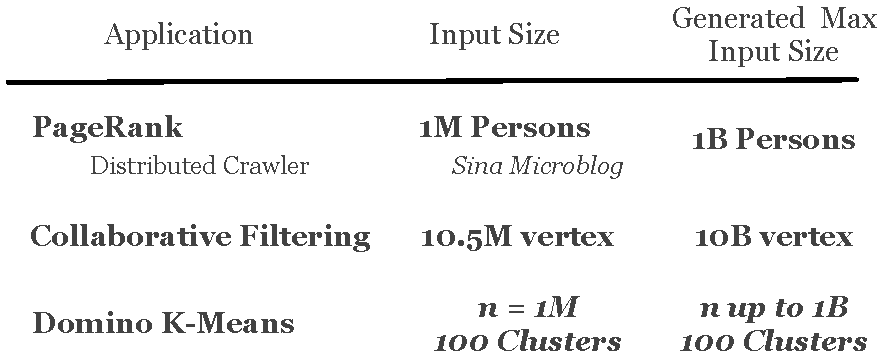
\includegraphics[width=4in]{data.pdf}
\caption{Domino相关测试输入数据大小}
\label{fig:data}
\end{figure}

\subsection{HBase性能比较}

按照我们之前的描述,Domino系统是基于对HBase的\textit{WAL}写动作进行监控实现的事件本地监测,并且通过向每一个\textit{RegionServer}添加本地周期扫描线程实现容错处理,除此之外,触发器的动作函数也是在HBase所运行的JVM中运行。因此这些操作一定会降低HBase本身的读写性能,本实验中我们将监测Domino实现本身对HBase系统性能的影响。本节所有实验都基于本地的9节点Domino集群实现。


\begin{figure}[h!]
  \centering
  \includegraphics[angle=270, width=4.5in]{gnuplot/cmphbase.eps}
  \caption{Domino和HBase写性能的对比图 1(Domino中无Trigger运行)}
  \label{cmphbase}
\end{figure}

\begin{figure}[h!]
  \centering
  \includegraphics[angle=270, width=4.5in]{gnuplot/cmphbaseouttrigger.eps}
  \caption{Domino和HBase写性能的对比图 2(Domino中Trigger高频率触发)}
  \label{cmphbase1}
\end{figure}

HBase的写性能测试中我们使用了\textit{PerformanceEvaluation}\cite{hbaseperformance}包,该包最早由HBase-399引入来测试HBase系统本身的读写性能。整个测试通过启动多个MapReduce任务完成,给定一个参数$n$,测试程序会在$n$台客户机上同时启动$10*n$个map任务,同时对HBase进行插入操作,每一个客户端将插入1百万行,每一行正好是1000字节。简单的计算可知,每一个map任务需要插入十万条。Reduce任务则比较简单,它会将所有的map中成功插入的条数做一个和,最后返回给用户。由于Reduce时间尽管没有对HBase进行写入,但依然会耗费大量的时间,因此在实际的比较中,我们将这一部分时间删去。为了更好的比较Domino和HBase的性能,我们根据整个MapReduce任务的执行时间计算出每一个map的平均执行时间,并且根据每一个map的平均写入条数来计算出单map的插入效率,通过乘以系统允许同时运行的map数目,最终得到整个HBase集群的写入速度。

图\ref{cmphbase}展示了当Domino中系统中没有触发器运行时与HBase的写性能的多次(共8次)试验的比较数据,此时所有的性能降低来自于我们的\textit{WAL Feeds}实现。我们发现Domino性能确有所降低,但是差别非常小(2\%)。图\ref{cmphbase1}则展示了当Domino系统中存在着频繁触发的触发器的时候系统的写性能与HBase的多次比较的结果。测试时我们对\textit{PreformanceEvaluation}所写的表设置了触发器,每次写入时,触发器都将执行。为了只检查触发本身的性能损失,触发器执行的动作非常简单,基本不占用CPU资源。从图中可以看出,即便在非常频繁的触发情况下,Domino和HBase相比性能下降依然在10\%以内。我们可以得出结论Domino本身实现带来的性能降低是非常小的。

\subsection{与MapReduce比较}

我们通过在Hadoop中实现了PageRank算法用以和Domino版本进行比较,而对于ALS算法和$k$-means算法我们采用了Mahout\cite{mahoutproject}中的实现。Mahout是一个基于Hadoop实现的饿开源大规模机器学习库,它包括了许多被高度优化的机器学习算法以及它们在Hadoop上基于MapReduce的实现。由于分布式爬虫没有任何可以基于MapReduce模型实现的必要,因此在本文中我们没有将其加入到比较中。

所有的实验都基于本地的9节点集群实现,所有的输入数据都是默认的输入数据,并且Domino使用了内存加速优化。在实验中,我们分别在3个节点和9个节点的集群上运行同样的应用以观察Domino应用和MapReduce应用的性能差别,以及进一步比较两种模型下应用的扩放性。从图\ref{spd}可以看出,在1百万个点的输入数据下,Domino的PageRank算法性能至少达到了基于Hadoop的PageRank实现的10倍以上的性能。而对于9个节点的集群来说,Domino下性能提升较Hadoop的提升也更大。

\begin{figure}[h!]
  \centering
  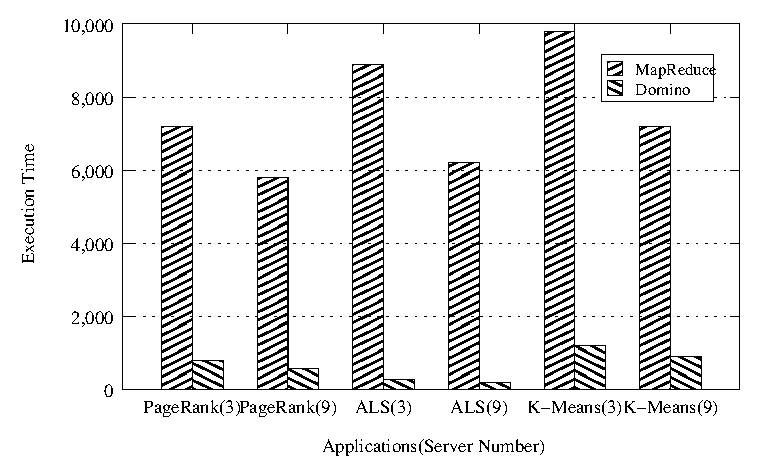
\includegraphics[width=5in]{gnuplot/cmpmapreduce.eps}
  \caption{PageRank、ALS、K-means算法的MapReduce实现和Domino实现的性能差别(3/9个节点)}
  \label{spd}
\end{figure}


从图\ref{spd}也可以看出ALS和$k$-means算法的性能提升同样非常明显,特别是ALS算法。这也很容易理解,由于Mahout中的ALS实现的每一个迭代包括了3个连续的MapReduce任务,这些MapReduce任务中所有的map函数并不进行计算,仅仅是为了将数据分发到不同的reduce函数中进行计算,这一切在Domino中都是不必须的,并且使用基于数据的模型是的Domino版本的ALS基本上不会进行多余的数据通讯。

\subsection{递增计算性能}

由于采用触发器模型,Domino模型最大的优势在于对递增计算的支持。PageRank的应用场景能够很好的体现这一点:通常情况下网络爬虫会不断的爬取新的网页交由PageRank进行排序。

\begin{figure}[h!]
  \centering
  \includegraphics[angle=270, width=5in]{gnuplot/increpr.eps}
  \caption{递增的PageRank在Domino和MapReduce下实现的性能对比}
  \label{incr}
\end{figure}

图\ref{incr}展示了Domino和MapReduce方案对于部分改变网页的计算性能对比。$y$轴表示了部分计算所花费的时间和全部都进行计算所花费时间的比率。基本的MapReduce语义中,无论几个页面发生了改变,为了得到正确的结果都需要对整个数据集运行一次完整的MapReduce程序。然而在Domino中,应用程序只需要对那些发生改变的页面以及与这些页面相关联的页面进行计算,因此Domino的递增计算性能远远好于MapReduce等系统:对于少量的输入数据集改变,可以立即得到新的结果。

\section{小结}
本章介绍了一个通用的基于触发器的编程模型及其运行时支持系统的设计和实现。通过引入聚合模式,我们在触发器这个纯异步模型的基础之上实现了同步语义;通过多版本数据管理,我们在Domino中引入了最终同步、严格同步模型,加上触发器本身的完全异步模型,为程序开发人员提供了针对应用可选的灵活模型。通过多种应用程序在Domino计算模型上的实现充分证明了该模型的有效性和通用性。除此之外,我们整合HBase存储系统实现了Domino运行时系统并且详细描述了各种优化策略,进一步提高其性能,应用的性能试验也证明了Domino运行时系统本身的高性能和高扩放性。Domino基于多版本数据管理为任务的容错和恢复设计了快速恢复的策略,能够有效的降低由于节点失效对整个应用执行速度的影响。

Domino并未对底层存储系统提出针对性的需求。带有容错和快速恢复功能的Domino仅要求底层存储系统能够提供数据持久化以及数据多版本存储的能力,因此Domino本身可以和多种存储系统整合起来以面向不同的应用场景。我们也正在进行这方面的工作,希望最终将存储系统和基于触发器编程模型模型紧密结合起来,作为云计算软件基础架构的核心组件存在。

